\documentclass[conference]{IEEEtran}
\IEEEoverridecommandlockouts
% The preceding line is only needed to identify funding in the first footnote. If that is unneeded, please comment it out.
\usepackage{cite}
\usepackage{amsmath,amssymb,amsfonts}
\usepackage{algorithmic}
\usepackage{graphicx}
\usepackage{textcomp}
\usepackage{xcolor}
\usepackage[utf8]{inputenc}
\usepackage[vietnamese]{babel}
\usepackage{amsmath}
\usepackage{float} % Sử dụng gói lệnh float để kiểm soát vị trí của hình ảnh

\def\BibTeX{{\rm B\kern-.05em{\sc i\kern-.025em b}\kern-.08em
    T\kern-.1667em\lower.7ex\hbox{E}\kern-.125emX}}
\begin{document}

\title{Conference Paper Title*\\
{\footnotesize \textsuperscript{*}Note: Sub-titles are not captured in Xplore and
should not be used}
\thanks{Identify applicable funding agency here. If none, delete this.}
}

\author{\IEEEauthorblockN{1\textsuperscript{st} Lê Thị Thanh Hằng}
\IEEEauthorblockA{\textit{dept. name of organization (of Aff.)} \\
\textit{name of organization (of Aff.)}\\
City, Country \\
email address or ORCID}
\and
\IEEEauthorblockN{2\textsuperscript{nd} Ngô Tất Tố}
\IEEEauthorblockA{\textit{dept. name of organization (of Aff.)} \\
\textit{name of organization (of Aff.)}\\
City, Country \\
email address or ORCID}
\and
\IEEEauthorblockN{3\textsuperscript{rd} Nguyễn Nhật Phương Huy}
\IEEEauthorblockA{\textit{dept. name of organization (of Aff.)} \\
\textit{name of organization (of Aff.)}\\
City, Country \\
email address or ORCID}
\and
\hspace{2cm}
\IEEEauthorblockN{4\textsuperscript{th} Lê Xuân Thạch}
\IEEEauthorblockA{\hspace{2.5cm}\textit{dept. Name of Organization (of Affiliation)} \\
\hspace{2.5cm}\textit{Name of Organization (of Affiliation)}\\
\hspace{2.5cm}City, Country \\
\hspace{2.5cm}Email Address or ORCID}
\and
\IEEEauthorblockN{5\textsuperscript{th} Hô Quang Đỉnh}
\IEEEauthorblockA{\textit{dept. name of organization (of Aff.)} \\
\textit{name of organization (of Aff.)}\\
City, Country \\
email address or ORCID}

}

\maketitle

\begin{abstract}
Nghiên cứu này đi sâu vào việc dự đoán giá của Heating Oil, Crude Oil WTI, Gasoline RBOB bằng cách sử dụng một loạt các thuật toán máy học và học sâu đa dạng. Chúng tôi sử dụng các mô hình Hồi quy tuyến tính, AIRMA, RNN, GRU, LSTM, FFT, DLM, FCN để đo độ chính xác và đáng tin cậy của các dự báo được tạo ra bởi mỗi thuật toán.
\end{abstract}

\begin{IEEEkeywords}
Time series analysis, Energy market investment, Forecasting gasoline and oil prices, machine learning, deep learning, LR, ARIMA, RNN, GRU, LSTM, FFT, DLM, FCN.\end{IEEEkeywords}

\section{Giới Thiệu}
Báo cáo này tập trung vào việc dự đoán giá cả trên thị trường dầu khí, tập trung vào ba loại dầu khí lớn: Heating Oil, Crude Oil WTI và Gasoline RBOB. Sử dụng các phương pháp phân tích chuỗi thời gian tiên tiến trên dữ liệu lịch sử, nghiên cứu nhằm mục đích phát hiện các mẫu và xu hướng giúp hiểu rõ hơn về biến động giá trong tương lai.

Mục đích của nghiên cứu này là hỗ trợ các nhà đầu tư, nhà phân tích tài chính và những người làm chính sách trong việc đưa ra quyết định thông minh về quản lý rủi ro, chiến lược đầu tư và kế hoạch tài chính.

Trong quá trình nghiên cứu, chúng tôi áp dụng một loạt các mô hình phân tích và dự đoán gồm Hồi quy Tuyến tính, ARIMA, RNN, GRU, LSTM, FFT, DLM, FCN và addRNN. Mỗi mô hình đều mang lại những ưu điểm riêng, giúp phân tích chi tiết các động lực phức tạp ảnh hưởng đến biến động giá cả của các loại dầu khí này.


\section{Các nghiên cứu liên quan}
Trong lĩnh vực dự đoán giá cổ phiếu hay thị trường chứng khoán, một số nghiên cứu quan trọng đã được tiến hành trên việc áp dụng các mô hình học máy.\\
T. Gopalakrishnan, R. Choudhary và S. Prasad, trong bài báo năm 2018 \cite{b1}, phân tích doanh số bán hàng của một siêu thị lớn và dự đoán doanh số bán hàng trong tương lai để giúp họ tăng lợi nhuận và làm cho thương hiệu của họ trở nên tốt hơn và cạnh tranh hơn theo xu hướng thị trường bằng cách tạo ra sự hài lòng cho khách hàng. Kỹ thuật được sử dụng để dự đoán doanh số bán hàng là thuật toán Hồi quy Tuyến tính. Dữ liệu doanh số bán hàng được thu thập từ năm 2011 đến 2013 và dự đoán cho năm 2014 được thực hiện. Sau đó, dữ liệu thời gian thực của năm 2014 cũng được thu thập và dữ liệu thực tế của năm 2014 đã được so sánh với dữ liệu dự đoán để tính toán độ chính xác của dự đoán. Điều này lại giúp họ thực hiện các hành động cần thiết (như đã được thảo luận sau) để tăng doanh số bán hàng của mình.\\
Benvenuto, D., Giovanetti, M., Vassallo, L., Angeletti, S., & Ciccozzi, M. trong nghiên cứu năm 2019 \cite{b2}. Áp dụng mô hình ARIMA trên bộ dữ liệu dịch CoVID-2019.Trung bình di chuyển tích hợp hồi quy tự động (ARIMA) trên dữ liệu dịch tễ học của Johns Hopkins để dự đoán xu hướng dịch tễ học về tỷ lệ lưu hành và tỷ lệ mắc bệnh COVID-2019. Để so sánh thêm hoặc để có tầm nhìn trong tương lai, việc xác định trường hợp và thu thập dữ liệu phải được duy trì theo thời gian thực.\\
Trong vài thập kỷ qua, nhiều khu vực đô thị trên thế giới đã phải hứng chịu tình trạng ô nhiễm không khí nghiêm trọng và các mối nguy hiểm sức khỏe đi kèm với nó, khiến việc thu thập chất lượng không khí theo thời gian thực và dự báo chất lượng không khí trở nên rất quan trọng để thực hiện các biện pháp phòng ngừa và khắc phục.Belavadi, S. V., Rajagopal, S., Ranjani, R., & Mohan, R. trong bài viết năm 2020.\cite{b3} Do thành tích đã được chứng minh là thành công với dữ liệu chuỗi thời gian,Long Short-Term Memory (LSTM) Recurrent Neural Network (RNN) mô hình được lựa chọn để thực hiện nhiệm vụ dự báo chất lượng không khí. Bài viết này phân tích một cách nghiêm túc hiệu suất của mô hình ở hai khu vực có sự khác biệt đáng kể về sự thay đổi theo thời gian của chất lượng không khí. Khi các biến thể này tăng lên, mô hình sẽ bị suy giảm hiệu suất, đòi hỏi phải có mô hình thích ứng.\\
Dự đoán năng lượng gió hiệu quả sẽ tạo điều kiện thuận lợi cho mục tiêu phát triển bền vững lâu dài của thế giới. Tuy nhiên, nhược điểm của gió với tư cách là nguồn năng lượng nằm ở tính biến thiên cao, dẫn đến việc nghiên cứu dự báo năng lượng gió gặp nhiều thách thức. Kisvari, A., Lin, Z., & Liu, X. vào năm 2021 đã có nghiên cứu \cite{b4} dự báo năng lượng gió bằng cách tích hợp tiền xử lý và lấy mẫu lại dữ liệu, phát hiện và xử lý các điểm bất thường, kỹ thuật tính năng và điều chỉnh siêu tham số dựa trên các mô hình học sâu định kỳ có kiểm soát, được thực hiện một cách có hệ thống. được trình bày lần đầu tiên. Bên cạnh đó, mạng lưới thần kinh học sâu mới của Gated Recurrent Unit (GRU) đã được phát triển thành công và được so sánh nghiêm túc với thuật toán Bộ nhớ ngắn hạn dài (LSTM). Ban đầu, 12 tính năng được thiết kế thành mô hình dự đoán, đó là tốc độ gió ở bốn độ cao khác nhau, nhiệt độ máy phát điện và nhiệt độ hộp số. Kết quả mô phỏng cho thấy, về mặt dự báo năng lượng gió, phương pháp đề xuất có thể đạt được độ chính xác cao với chi phí tính toán thấp hơn. Cũng có thể kết luận rằng GRU vượt trội hơn LSTM về độ chính xác dự đoán trong tất cả các thử nghiệm được quan sát, mang lại quy trình đào tạo nhanh hơn và ít nhạy cảm hơn với nhiễu trong bộ dữ liệu Kiểm soát giám sát và Thu thập dữ liệu (SCADA) đã sử dụng.\\
Hiện nay, ùn tắc giao thông đã trở thành một phần trong cuộc sống hàng ngày của người dân ở các thành phố trên khắp thế giới và tác động tiêu cực đến cuộc sống của người dân, ví dụ như mất thêm thời gian đi lại, tăng lượng khí thải, v.v. Để giảm thiểu tác động của tắc nghẽn giao thông đối với cuộc sống của chúng ta, những nỗ lực nghiên cứu chuyên sâu đã được đề xuất về vấn đề này.\cite{b5}
Nền kinh tế Ấn Độ và sản xuất ngũ cốc có mối liên hệ chặt chẽ với sự phân bố không gian và lượng mưa trong thời kỳ gió mùa mùa hè (tháng 6 đến tháng 9). Nhiều nghiên cứu đã đi sâu vào các phương pháp mô hình hóa để dự báo lượng mưa gió mùa mùa hè ở Ấn Độ. K. V. Narasimha Murthy, G. Kishore Kumar & P. N. Sen đã sử dụng dữ liệu lượng mưa hàng tháng trong 72 năm (1950–2021) để phân tích, lập mô hình và dự đoán gió mùa ở Tây Bắc Ấn Độ bằng Mô hình tuyến tính động (DLM).\cite{b6}\\
C. Hecht; R. Aghsaee; F. Schwinger; J. Figgener; M. Jarke; D. U. Sauer đã Dự đoán ngắn hạn về tính khả dụng của trạm sạc xe điện bằng cách sử dụng mô hình học máy xếp tầng. \cite{b7}\\
Vào năm 2023, G Kalpana - Mukt Shabd Journal dự báo chuỗi thời gian và mô hình hóa chuỗi cung ứng nhu cầu thực phẩm dựa trên phân tích hồi quy.\cite{b8} \\
\section{Bộ dữ liệu}

\subsection{Nguồn dữ liệu}

- Bộ dữ liệu này bao gồm giá bán trong ngày của 3 loại nhiên liệu phổ biến tại Hoa Kỳ từ 1/1/2019 đến 27/3/2024. Dữ liệu được thu thập từ trang web investing.com, một nguồn tin cậy và uy tín trong lĩnh vực tài chính.

+ Dầu sưởi ấm (Heating Oil): Là loại nhiên liệu lỏng được sử dụng để sưởi ấm nhà cửa và các tòa nhà trong mùa đông. Do nhu cầu sưởi ấm tăng cao vào mùa lạnh, giá dầu sưởi ấm thường biến động theo mùa.

+ Dầu thô WTI (Crude Oil WTI): Là loại dầu thô nhẹ đóng vai trò tiêu chuẩn cho giá dầu thô trên toàn thế giới. Giá dầu WTI chịu ảnh hưởng bởi nhiều yếu tố, bao gồm cung cầu, chính sách chính phủ, và các sự kiện địa chính trị.

+ Xăng RBOB (Gasoline RBOB): Là loại xăng được pha chế để đáp ứng các tiêu chuẩn về môi trường, sử dụng cho các phương tiện giao thông chạy bằng động cơ đốt trong. Giá xăng RBOB thường biến động theo giá dầu WTI và các yếu tố khác như thuế, phí.

- Mô tả các thành phần của tập dữ liệu:

Date:

+ Ý nghĩa: Ngày dữ liệu được ghi nhận

+ Kiểu dữ liệu: Datetime

Price:

+ Ý nghĩa: Giá cuối cùng của ngày giao dịch đó

+ Kiểu dữ liệu: Float

Open:

+ Ý nghĩa: Giá đầu tiên được giao dịch trong ngày đó

+ Kiểu dữ liệu: Float

High:
+ Ý nghĩa: Giá cao nhất được giao dịch trong ngày

+ Kiểu dữ liệu: Float

Low:

+ Ý nghĩa: Giá thấp nhất được giao dịch trong ngày

+ Kiểu dữ liệu: Float

Vol (volume):

+ Ý nghĩa: Tổng số lượng nhiên liệu được giao dịch trong ngày

+ Kiểu dữ liệu: Float

Change \%:

+ Ý nghĩa: Phần trăm thay đổi giữa giá cuối cùng của ngày dữ liệu ghi nhận so với ngày trước đó

+ Kiểu dữ liệu: Float

\subsection{Thống kê mô tả}
\begin{table}[H]
  \centering
  \caption{Heating Oi, Crude Oil WTI, Gasoline RBOB’s Descriptive Statistics}
\begin{tabular}{|>{\columncolor{red!20}}c|c|c|c|}
    \hline
     \rowcolor{red!20} & HT Oil& WTI& RBOB\\ \hline
     Count & 1320
& 1322
& 1550
\\ \hline
     Mean & 2.351011
& 68.126384
& 1.946561
\\ \hline
     Std & 0.846315
& 20.452117
& 0.590874
\\ \hline
     Min & 0.6104
& -37.63
& 0.543
\\ \hline
     25\% & 1.8314
& 55.705
& 1.411925
\\ \hline
     50\% & 2.15365
& 70.015
& 1.9412
\\ \hline
     75\% & 2.891425
& 80.5
& 2.44925
\\ \hline
     Max & 5.1354
& 123.7
& 4.3144
\\ \hline
 Mode& 3.3622
& 47.62
&2.581
\\\hline
 Median& 2.15365
& 70.015
&1.9412
\\\hline
 Var& 0.716249
& 418.289074
&0.349132
\\\hline
 Kurtosis& -0.39922
& 0.452915
&-0.377936
\\\hline
 Skewness& 0.389108
& -0.09777
&0.261192
\\\hline
 CV& 0.359979
& 0.300208
&0.303548
\\\hline
\end{tabular}
\end{table}

\begin{figure}[H]
    \centering
    \begin{minipage}{0.23\textwidth}
    \centering
    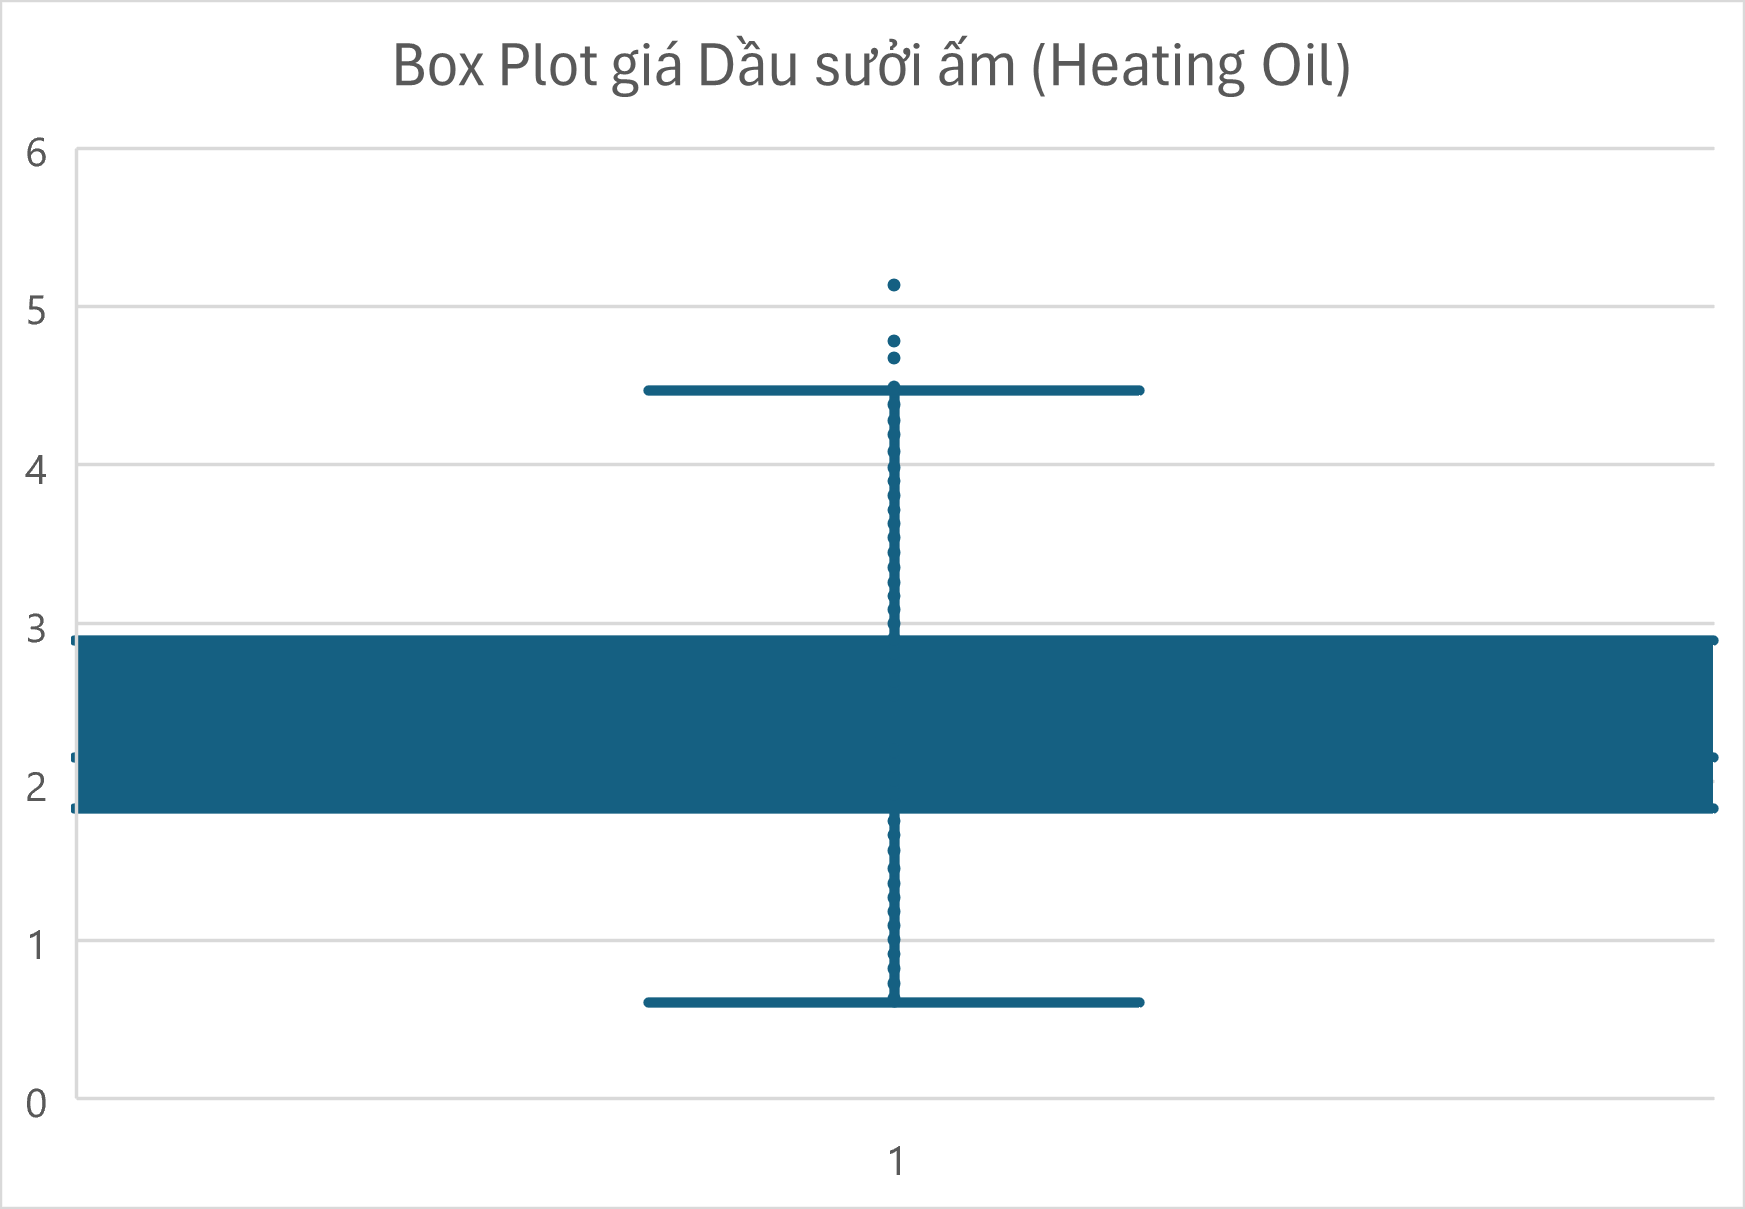
\includegraphics[width=1\textwidth]{Picture/BoxPlot cho phần III/Team9_Box_HeatingOil.png}
    \caption{Box Plot giá Dầu sưởi ấm (Heating Oil)}
    \label{fig:1}
    \end{minipage}
    \hfill
    \begin{minipage}{0.23\textwidth}
    \centering
    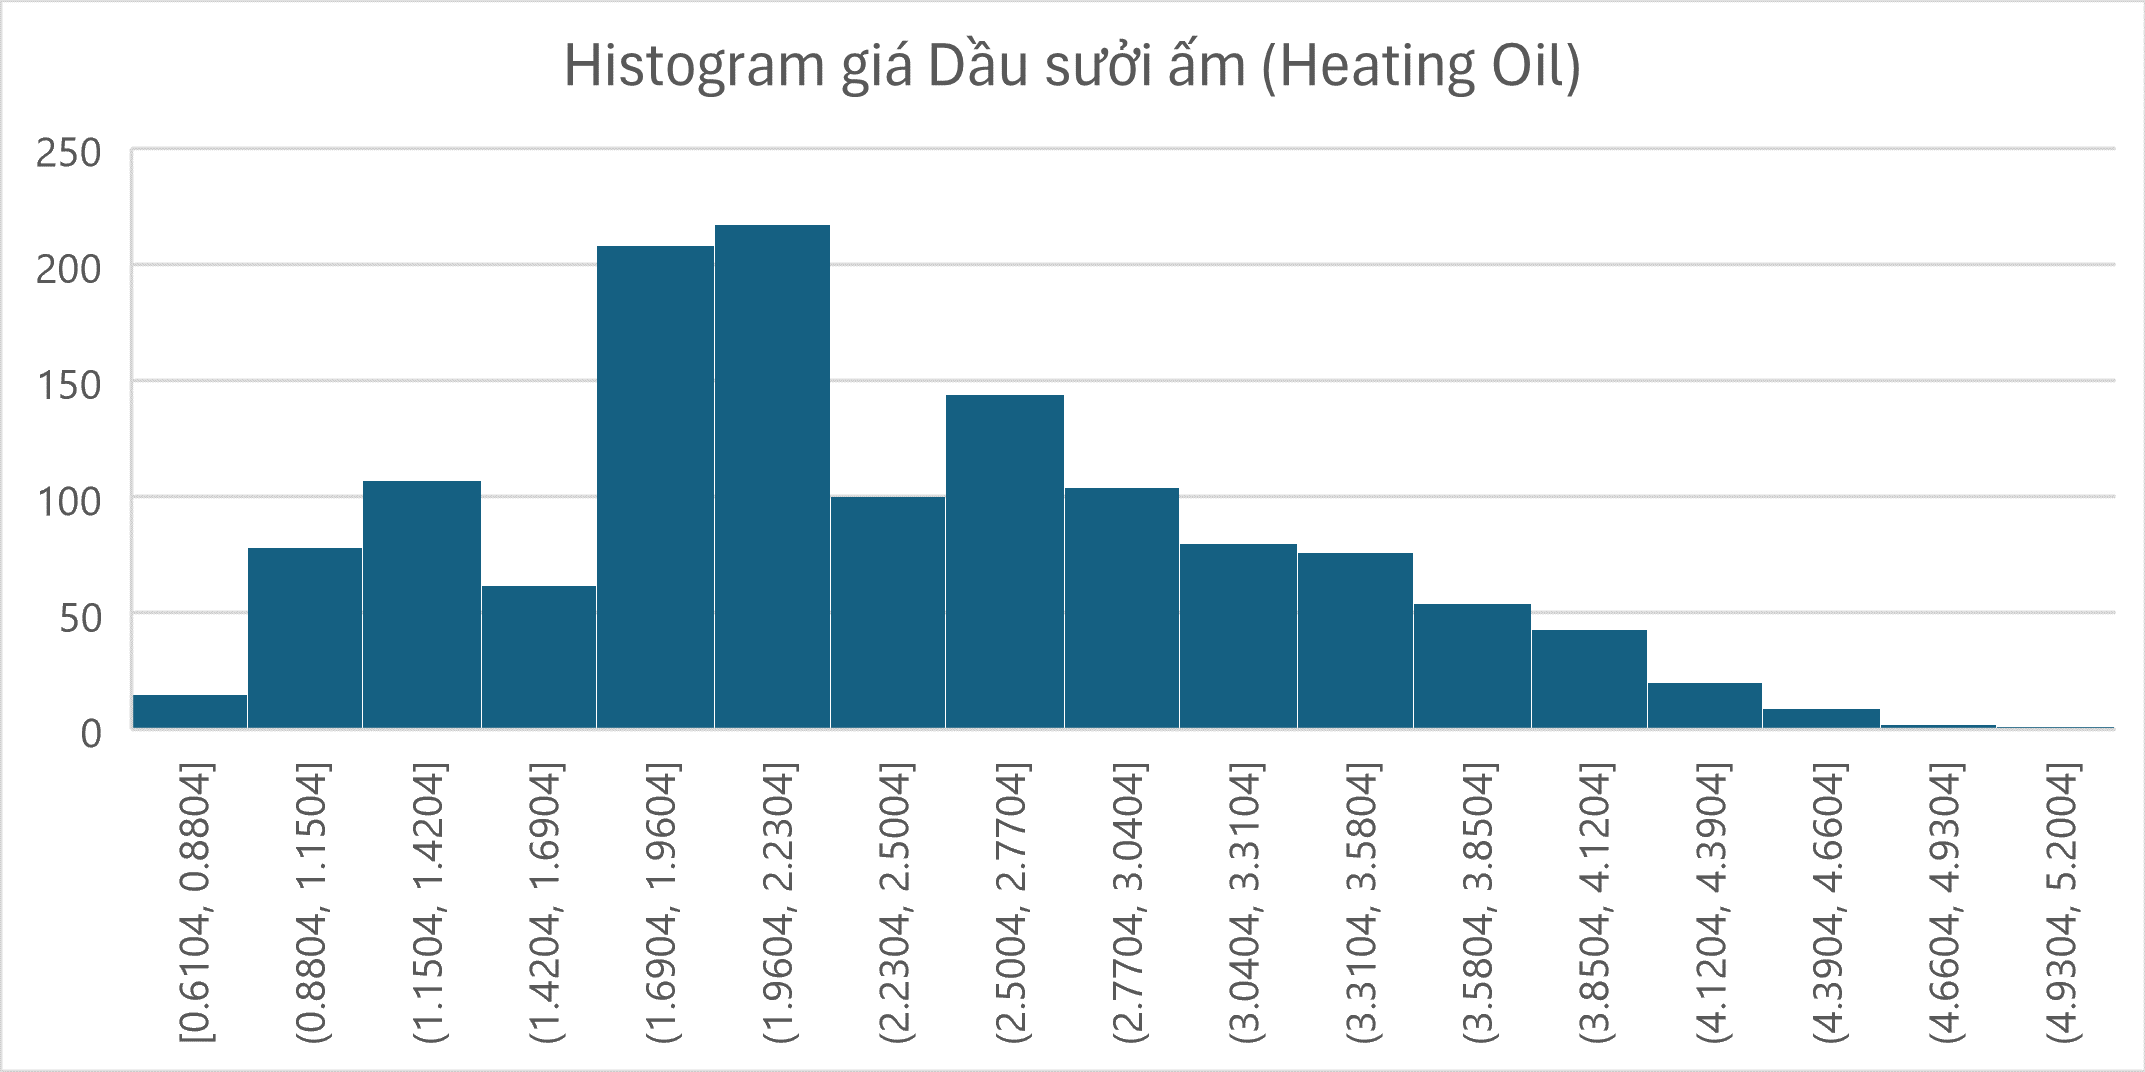
\includegraphics[width=1\textwidth]{Picture/Histogram cho ở phần III/Team9_His_HeatingOil.png}
    \caption{Histogram giá Dầu sưởi ấm (Heating Oil)}
    \label{fig:2}
    \end{minipage}
\end{figure}

\begin{figure}[H]
    \centering
    \begin{minipage}{0.23\textwidth}
    \centering
    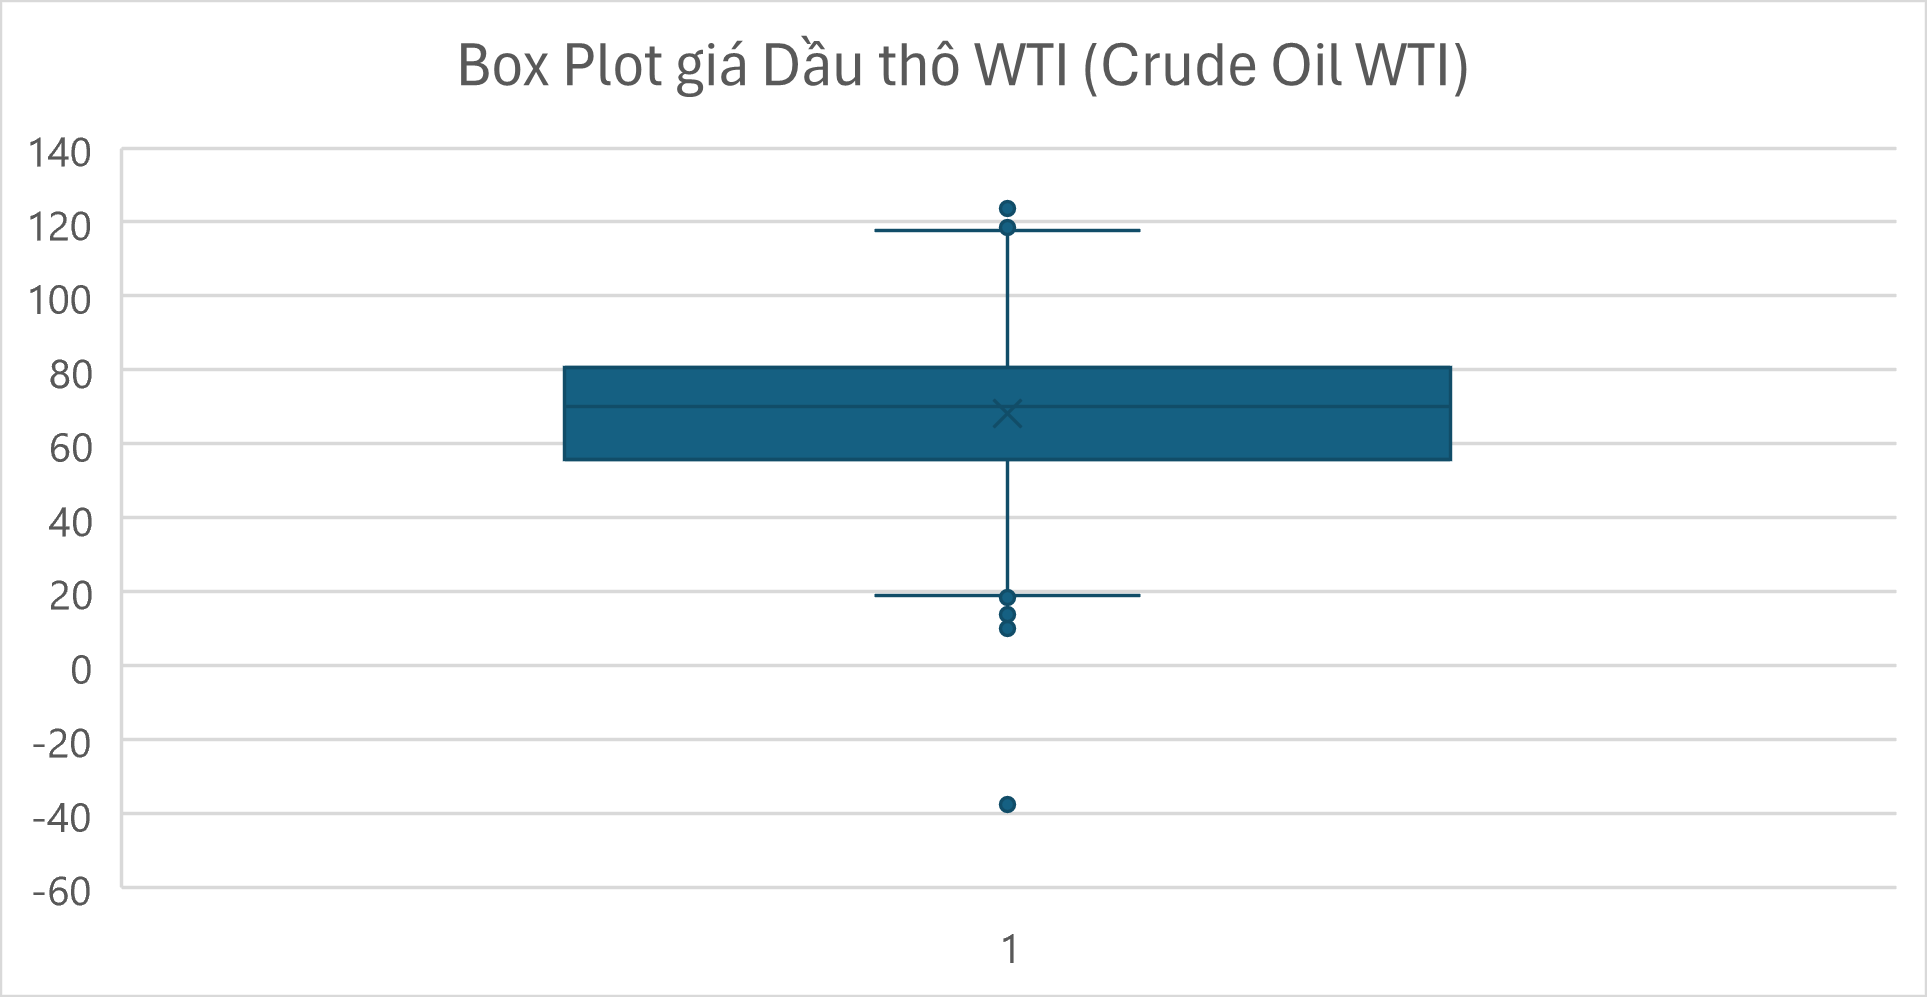
\includegraphics[width=1\textwidth]{Picture/BoxPlot cho phần III/Team9_Box_WTI.png}
    \caption{Boxplot giá Dầu thô WTI (Crude Oil WTI}
    \label{fig:1}
    \end{minipage}
    \hfill
    \begin{minipage}{0.23\textwidth}
    \centering
    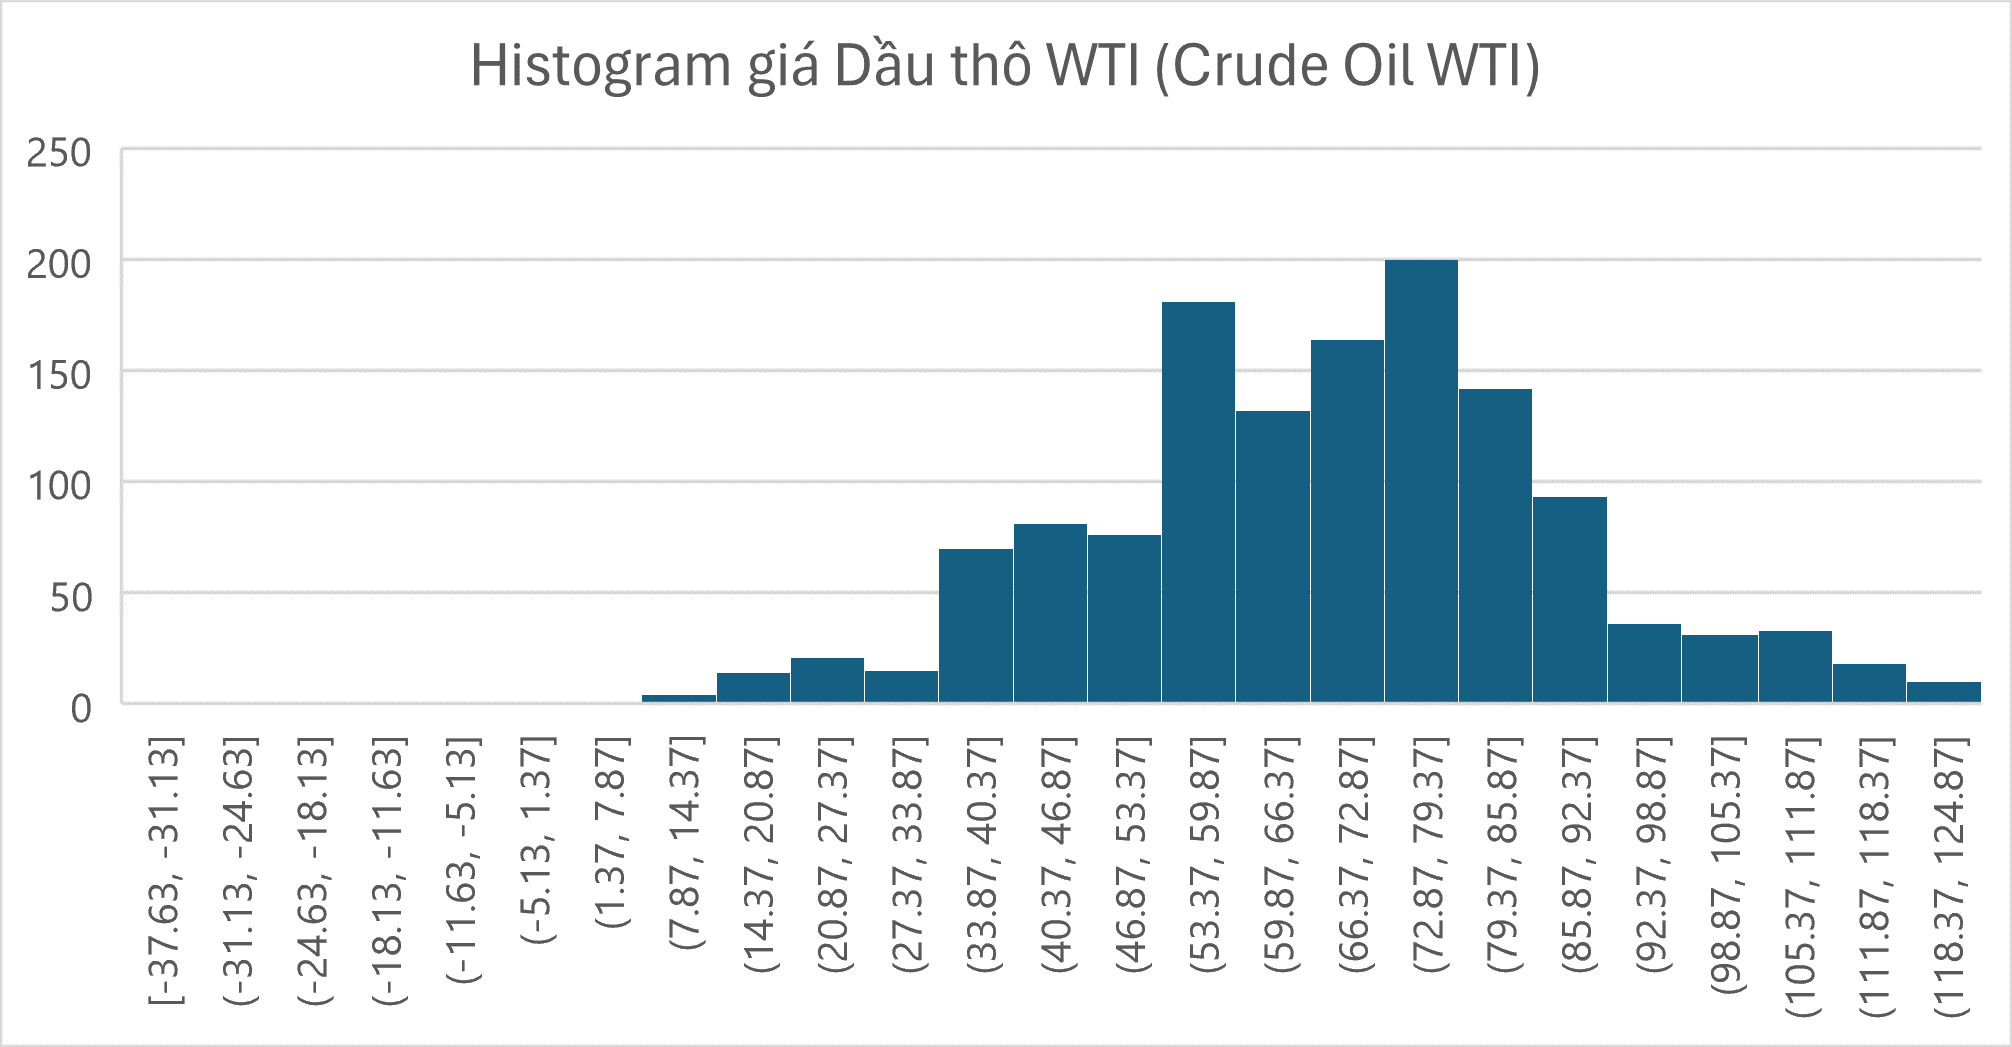
\includegraphics[width=1\textwidth]{Picture/Histogram cho ở phần III/Team9_His_WTI.png}
    \caption{Histogram giá Dầu thô WTI (Crude Oil WTI)}
    \label{fig:2}
    \end{minipage}
\end{figure}

\begin{figure}[H]
    \centering
    \begin{minipage}{0.23\textwidth}
    \centering
    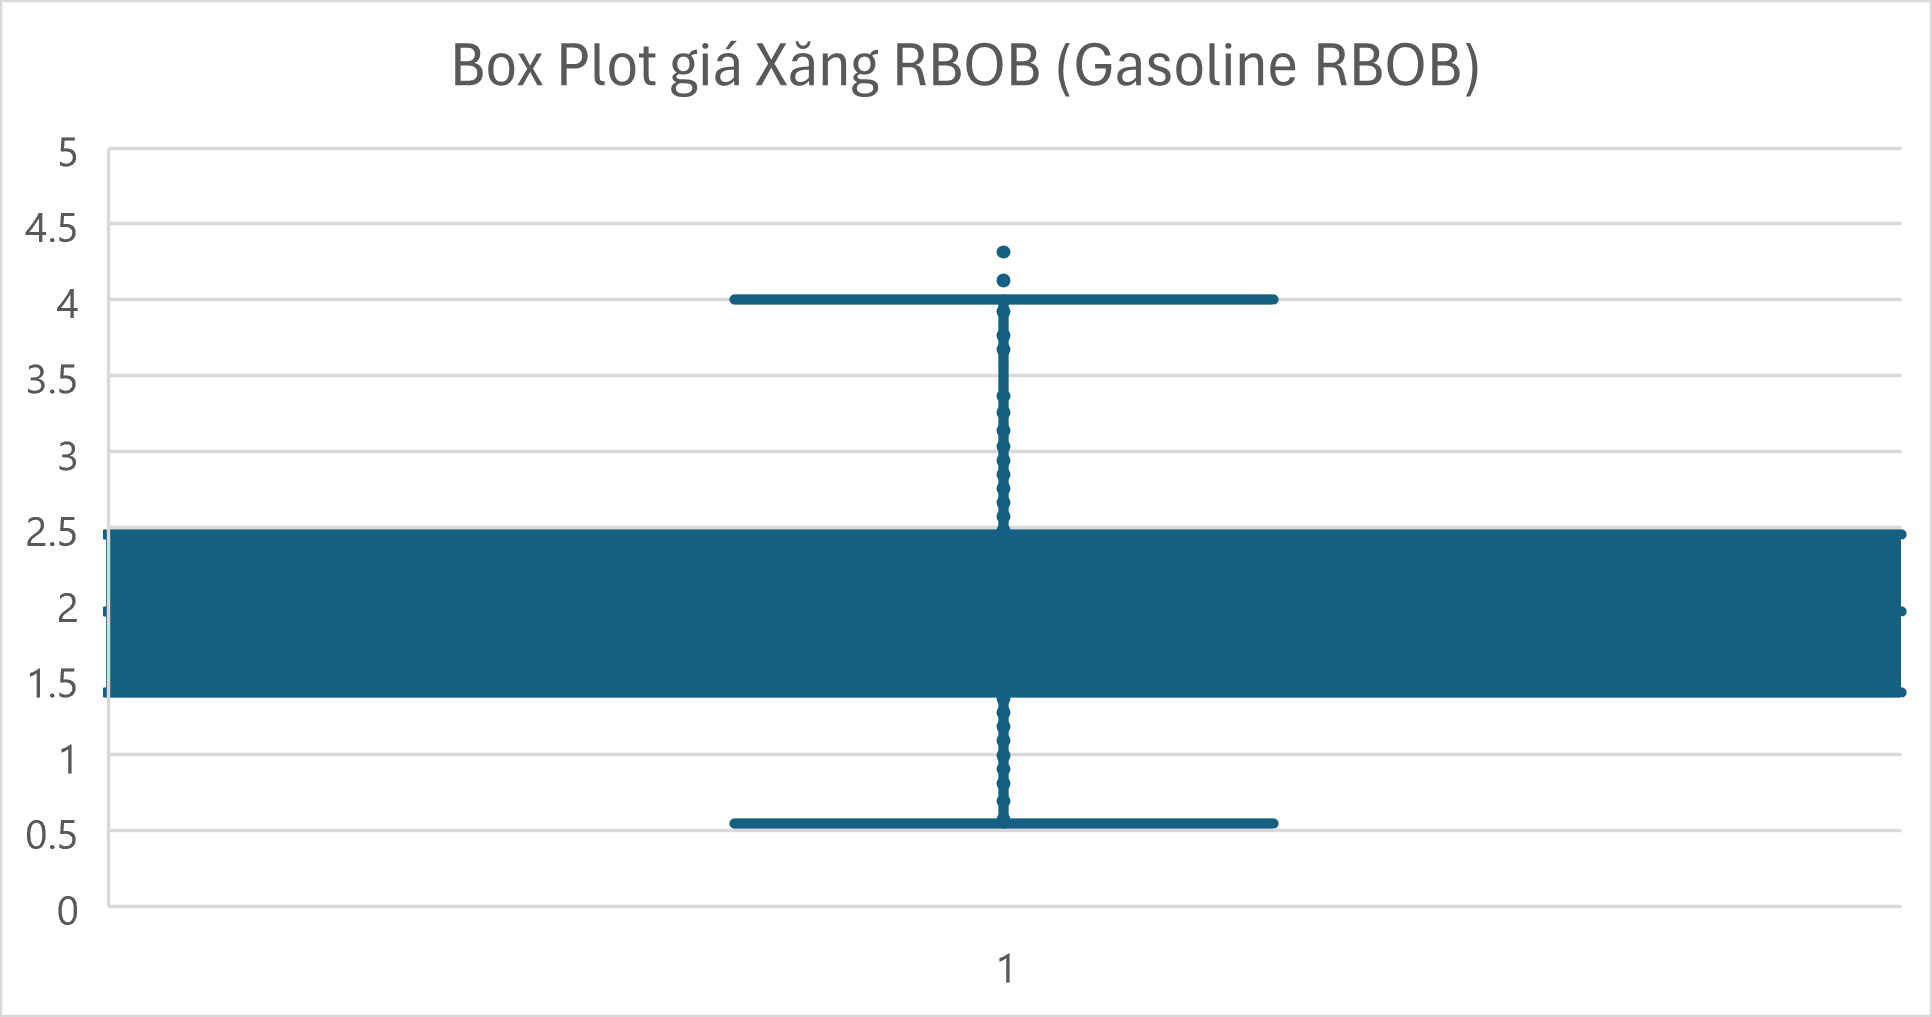
\includegraphics[width=1\textwidth]{Picture/BoxPlot cho phần III/Team9_Box_RBOB.png}
    \caption{Boxplot giá Xăng RBOB (Gasoline RBOB)}
    \label{fig:1}
    \end{minipage}
    \hfill
    \begin{minipage}{0.23\textwidth}
    \centering
    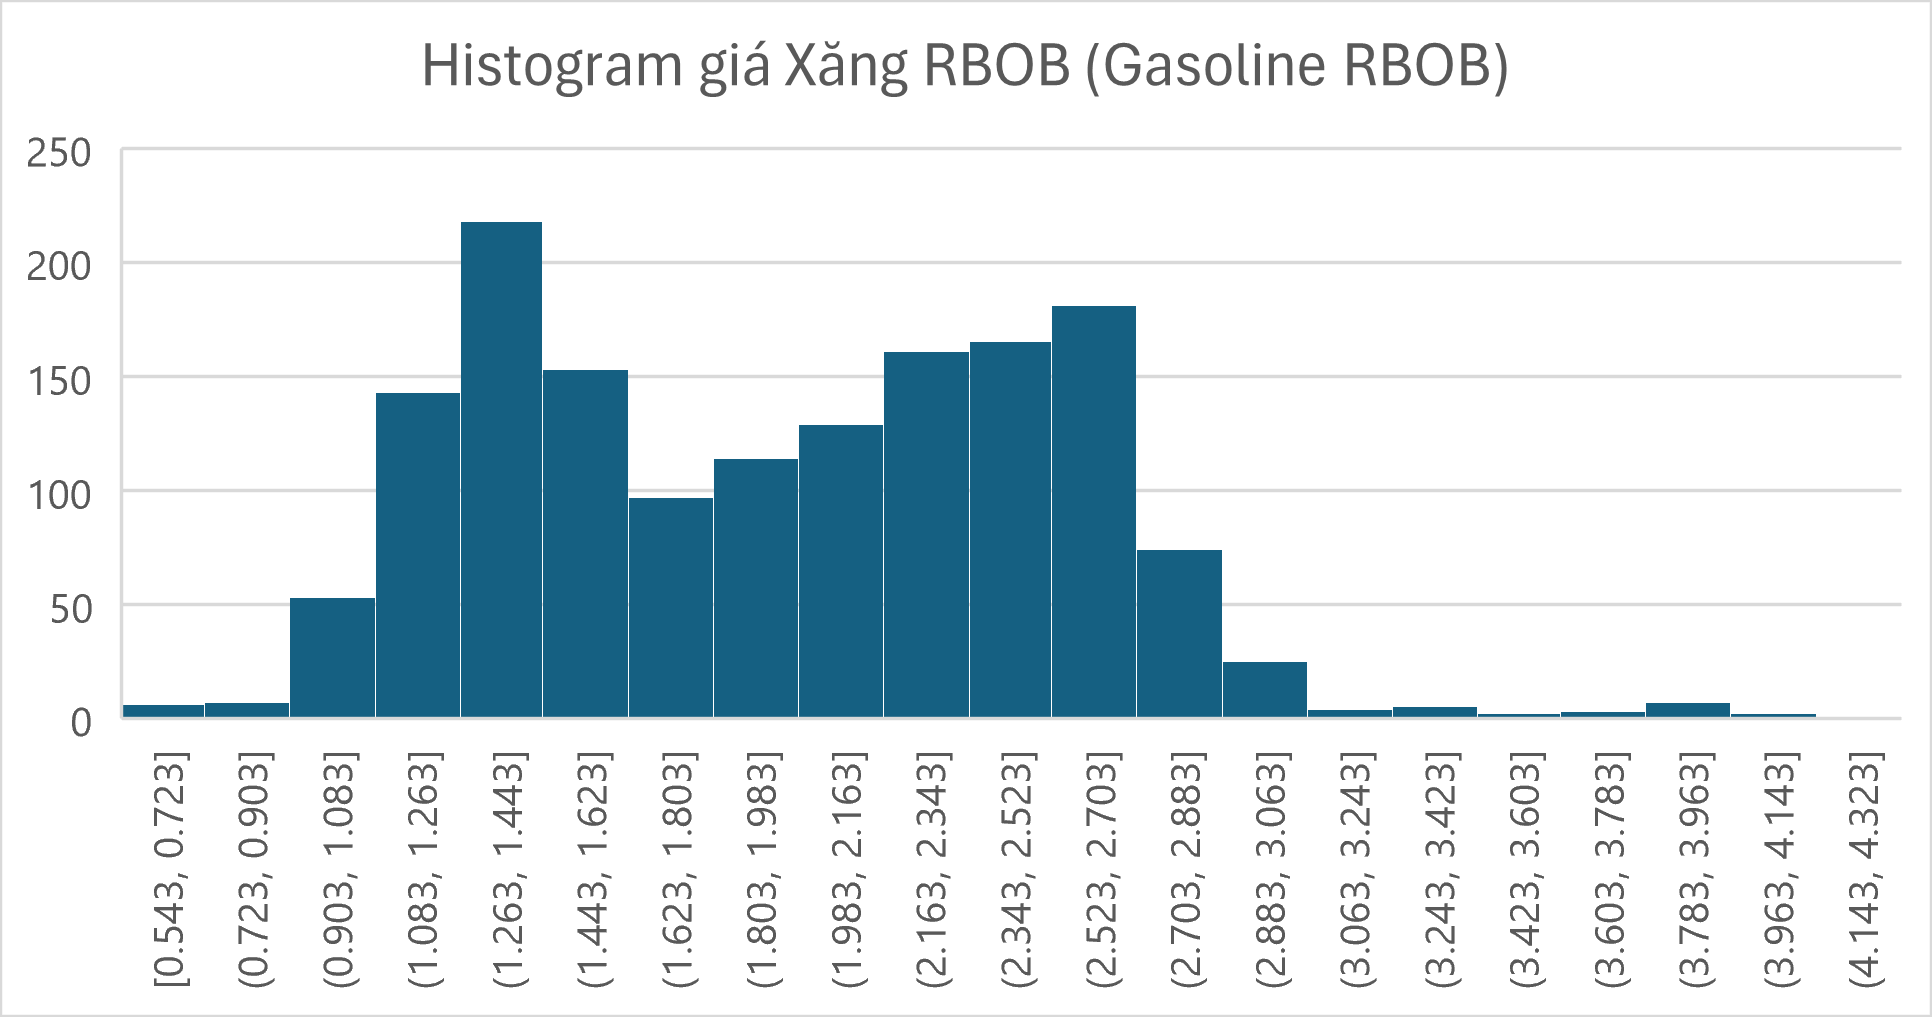
\includegraphics[width=1\textwidth]{Picture/Histogram cho ở phần III/Team9_His_RBOB.png}
    \caption{Histogram giá Xăng RBOB (Gasoline RBOB)}
    \label{fig:2}
    \end{minipage}
\end{figure}
\subsection{Công cụ}
Trong quá trình nghiên cứu và phân tích dữ liệu, nhóm đã sử dụng một bộ công cụ phân tích thống kê bằng Python để hiểu sâu hơn về các mẫu dữ liệu và rút ra ý nghĩa, kết luận. Các công cụ chính bao gồm: numpy, pandas, sklearn, matplotlib.pyplot,...


\subsection{Tỉ lệ phân chia dữ liệu}
    Trong việc phân tích dữ liệu chuỗi thời gian, nhóm đã chia tập dữ liệu thành các tập huấn luyện và kiểm tra bằng các tỷ lệ khác nhau: 70\% cho huấn luyện và 30\% cho kiểm tra, 80\% cho huấn luyện và 20\% cho kiểm tra, 90\% cho huấn luyện và 10\% cho kiểm tra. 

Những tỷ lệ này cho phép đánh giá tác động của các chỉ số liên quan đến hiệu suất của mô hình bằng cách xem xét phân phối dữ liệu trong mỗi tập. Tỷ lệ phổ biến 7:3 phân bổ 70\% cho huấn luyện và 30\% cho kiểm tra, tạo ra một sự cân bằng giữa cung cấp đủ dữ liệu huấn luyện, đồng thời đảm bảo sự khác nhau giữa các tập cho việc điều chỉnh và đánh giá. Một lựa chọn khác là tỷ lệ 8:2, ưu tiên tập huấn luyện 80\%, có lợi cho các mô hình phức tạp yêu cầu một tập dữ liệu huấn luyện lớn hơn. Hoặc một cách phân tích thận trọng dùng tỷ lệ 9:1 có thể được ưa chuộng, khi xử lý một tập dữ liệu lớn và một mô hình đơn giản. Tỷ lệ này đảm bảo dữ liệu huấn luyện và vẫn đủ dữ liệu một tập kiểm tra để đánh giá hiệu suất.

\subsection{Đánh giá mô hình}
RMSE được tính bằng cách lấy căn bậc hai của trung bình cộng bình phương của các sai số (khác biệt giữa giá trị dự đoán và giá trị thực tế) giữa một loạt các điểm dữ liệu. RMSE càng nhỏ thì mô hình dự đoán càng chính xác.

MAPE được tính bằng cách lấy trung bình cộng của tỷ lệ tuyệt đối giữa sai số tuyệt đối và giá trị thực tế cho mỗi điểm dữ liệu, sau đó nhân 100 để biểu diễn dưới dạng phần trăm.

MAE được tính bằng cách lấy trung bình cộng của các giá trị tuyệt đối của sai số giữa giá trị dự đoán và giá trị thực tế.

\[RMSE=\sqrt{\sum_{i=1}^{n} \frac{(\hat{y_i}-y_i )^2}{n} }\]\\

\[MAPE = \frac{1}{n} \sum_{i=1}^{n} \left| \frac{y_i - \hat{y_i}}{y_i} \right| \times 100\]\\

\[MAE = \frac{1}{n} \sum_{i=1}^{n} \left| y_i - \hat{y_i} \right|]\\

Trong đó: \\
	\indent\textbullet\ \(n\) là số lượng các điểm dữ liệu.
 
	\indent\textbullet\ \(y_i\)  là các giá trị thực tế của điểm dữ liệu thứ i.
 
	\indent\textbullet\ \(\hat{y_i}\) là các giá trị dự đoán của điểm dữ liệu thứ i.



\section{Phương pháp thống kê}
\subsection{Linear Regression}
Phân tích hồi quy là một phân tích thống kê để xác định xem quan hệ các biến độc lập quy định các biến phụ thuộc như thế nào.\\
Hồi quy tuyến tính là một công cụ dùng để xây dựng các mô hình toán học và thống kê, mô tả mối quan hệ giữa biến phụ thuộc và một hoặc nhiều biến độc lập (hoặc biến giải thích), tất cả đều là các biến số.Mô hình hồi quy tuyến tính này được sử dụng để tìm phương trình dự đoán tốt nhất cho biến y dưới dạng một hàm tuyến tính của các biến x\\

Mô hình hồi quy tuyến tính bội có dạng: 
\[Y=\beta_0+\beta_1X_1+\beta_2X_2+\cdots+\beta_kX_k+\varepsilon\]
Định Nghĩa:\\
	\indent\textbullet\ Y là biến phụ thuộc (biến mục tiêu).\\
	\indent\textbullet\ \(X_1, X_2, \ldots, X_k\) là các biến độc lập (biến giải thích).\\
	\indent\textbullet\ \(\beta_0\) là giá trị trung bình của biến phụ thuộc khi x=0.\\
	\indent\textbullet\ \(\beta_1,..., \beta_k\) là các hệ số cho các biến độc lập.\\
	\indent\textbullet\ \(\varepsilon\) là sai số của mô hình.
 \\
\begin{figure}[H]
    \centering
    \begin{minipage}{0.3\textwidth}
    \centering
    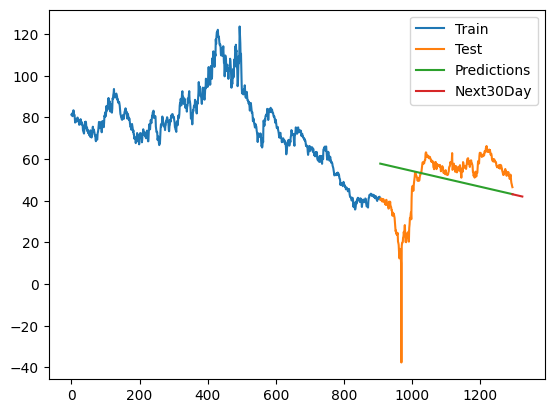
\includegraphics[width=0.8\textwidth]{Picture/LinearRegression/LinearRegressSion(Cruide_7_3).png} 
    \caption{Crude Oil WTI 7:3}
    \label{fig:1}
    \end{minipage}
    \hfill
    \\
    \begin{minipage}{0.3\textwidth} 
    \centering
    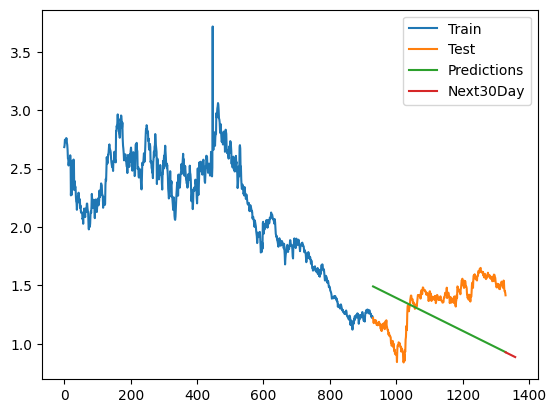
\includegraphics[width=0.8\textwidth]{Picture/LinearRegression/LinearRegressSion(GasOline_7_3).png} 
    \caption{Gasoline RBOB 7:3}
    \label{fig:2}
    \end{minipage}
    \hfill
    \\
    \begin{minipage}{0.3\textwidth}
    \centering
    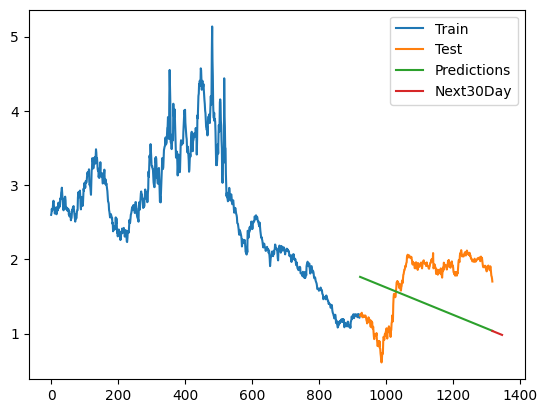
\includegraphics[width=0.8\textwidth]{Picture/LinearRegression/LinearRegressSion(HeatingOil_7_3).png}
    \caption{Heating Oil 7:3}
    \label{fig:3}
    \end{minipage}
\end{figure}


 
   
\subsection{ARIMA}
 ARIMA (Auto-Regressive Integrated Moving-Average) là mô hình phân tích thống kê sử dụng dữ liệu chuỗi thời gian để hiểu rõ hơn về tập dữ liệu hoặc để dự đoán xu hướng trong tương lai. Trong phần này sẽ đề cập về ARIMA không có tính mùa vụ (Non-seasonal).
 
 Mô hình ARIMA không có tính mùa vụ (Non-seasonal) được kí hiệu là ARIMA(p,d,q) với p, d, q là các số không âm. Trong đó, ARIMA bao gồm 3 phần:
 
 \indent\textbullet\ \textbf{AR(p)} - \textit{Auto-Regression}: là quá trình tìm mối quan hệ giữa dữ liệu hiện tại và \textbf{\textit{p}} dữ liệu trước đó (hay còn gọi là lag). Mô hình AR(p) có dạng:
 \[y_t = \alpha_0 + \alpha_1 y_{t-1} + \alpha_2 y_{t-2} + \cdots + \alpha_p y_{t-p} + \varepsilon_t\]

Trong đó, điều kiện dừng của việc chọn \textbf{\textit{p}} là: $\sum_{i=0}^{p} \alpha_i < 1$ \\

 \indent\textbullet\ \textbf{MA(q)} - \textit{Moving-Average}: là quá trình tìm mối quan hệ giữa dữ liệu hiện tại và \textbf{\textit{q}} phần lỗi trước đó. Mô hình MA(q) có dạng: 
\[y_t = \beta_0 + \beta_1 \varepsilon_{t-1} + \beta_2 \varepsilon_{t-2} + \cdots + \beta_q \varepsilon_{t-q} + \mu_t\]

 Trong đó, điều kiện dừng của việc chọn \textbf{\textit{q}} là: $\sum_{i=0}^{q} \beta_i < 1$ \\

 \indent\textbullet\ \textbf{I(d)} - \textit{Integrated}: là quá trình đồng tích hợp hoặc lấy sai phân. Để tạo thành chuỗi dừng cho mô hình ARMA, một cách đơn giản nhất là lấy sai phân (I - Integrated) để tạo thành mô hình ARIMA. Với \textbf{\textit{d}} là số chênh lệch cần thiết cho tính dừng (hiệu giữa giá trị hiện tại và \textbf{\textit{d}} giá trị trước đó).

 Quá trình sai phân bậc \textbf{\textit{d}} (hoặc \textbf{\textit{d}} lần lấy sai phân) của chuỗi được thực hiện như sau:\\
 Sai phân bậc 1 - I(1): $\Delta y_t = y_t - y_{t-1}$  \\
 Sai phân bậc 2 - I(2): $\Delta(\Delta y_t) = (y_t - y_{t-1}) - (y_{t-1} - y_{t-2}) $ \\
 Sai phân bậc \textbf{\textit{d}} - I(d): $\Delta^d (x_t)$\\

\begin{figure}[H]
    \centering
    \begin{minipage}{0.3\textwidth}
    \centering
    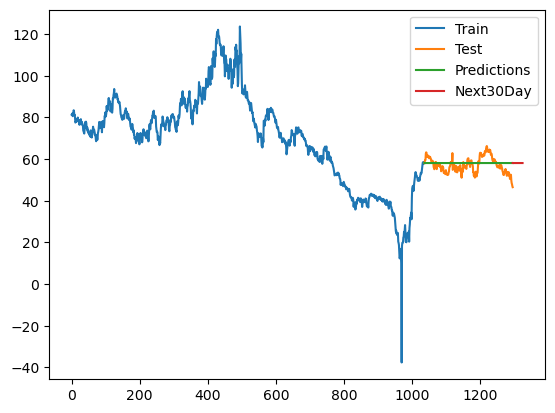
\includegraphics[width=0.8\textwidth]{Picture/ARIMA/Crude Oil WTI 8-2.png} 
    \caption{Crude Oil WTI 8:2}
    \label{fig:1}
    \end{minipage}
    \hfill
    \\
    \begin{minipage}{0.3\textwidth} 
    \centering
    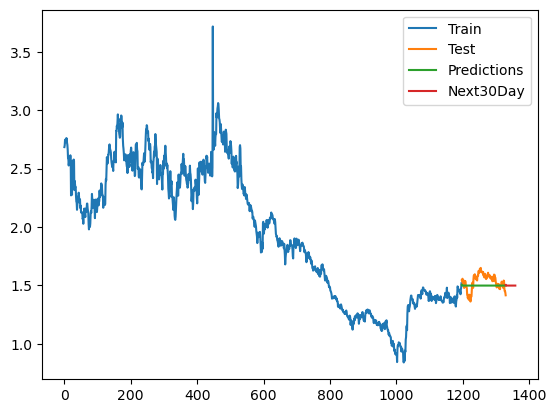
\includegraphics[width=0.8\textwidth]{Picture/ARIMA/Gasoline RBOB 9-1.png} 
    \caption{Gasoline RBOB 9:1}
    \label{fig:2}
    \end{minipage}
    \hfill
    \\
    \begin{minipage}{0.3\textwidth}
    \centering
    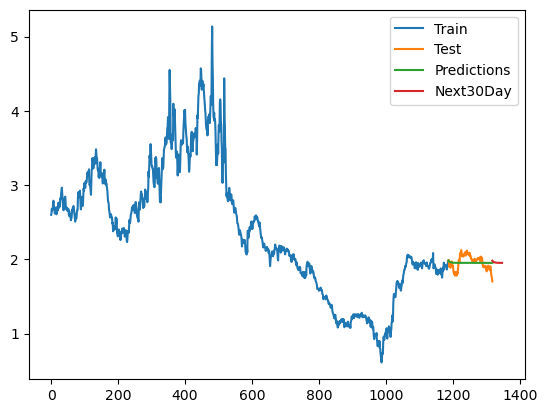
\includegraphics[width=0.8\textwidth]{Picture/ARIMA/Heating Oil 9-1.png}
    \caption{Heating Oil 9:1}
    \label{fig:3}
    \end{minipage}
\end{figure}

\subsection{Fast Fourier Transform Forecasting Model (FFT)}
Fast Fourier Transform - FFT là một thuật toán được sử dụng để dự đoán các giá trị dữ liệu trong tương lai. Thuật toán này biến đổi Fourier rời rạc của một dãy hoặc nghịch đảo của nó, thường thì cả hai đều được thực hiện. Phân tích Fourier biến đổi tín hiệu từ miền của dữ liệu đã cho, thường là thời gian hoặc không gian, và biến đổi nó thành biểu diễn tần số.


Công thức của thuật toán FFT:
 \[
X_k = \sum_{m=0}^{N/2-1} x_{2m}e^{-\frac{2\pi i}{N}mk} + \sum_{m=0}^{N/2-1} x_{2m+1}e^{-\frac{2\pi i}{N}(m+N/2)k}
\]

Trong đó:

\begin{itemize}
    \item \( X_k \): Giá trị của Fourier tại vị trí \( k \).
    \item \( x_m \): Giá trị của điểm dữ liệu trong dữ liệu đầu vào tại vị trí \( m \).
    \item \( N \): Kích thước của dữ liệu đầu vào.
    \item \( e \): Số Euler, một hằng số toán học (\( e \approx 2.71828 \)).
    \item \( i \): Đơn vị ảo trong toán học.
\end{itemize}

\begin{figure}[H]
    \centering
    \begin{minipage}{0.3\textwidth}
    \centering
    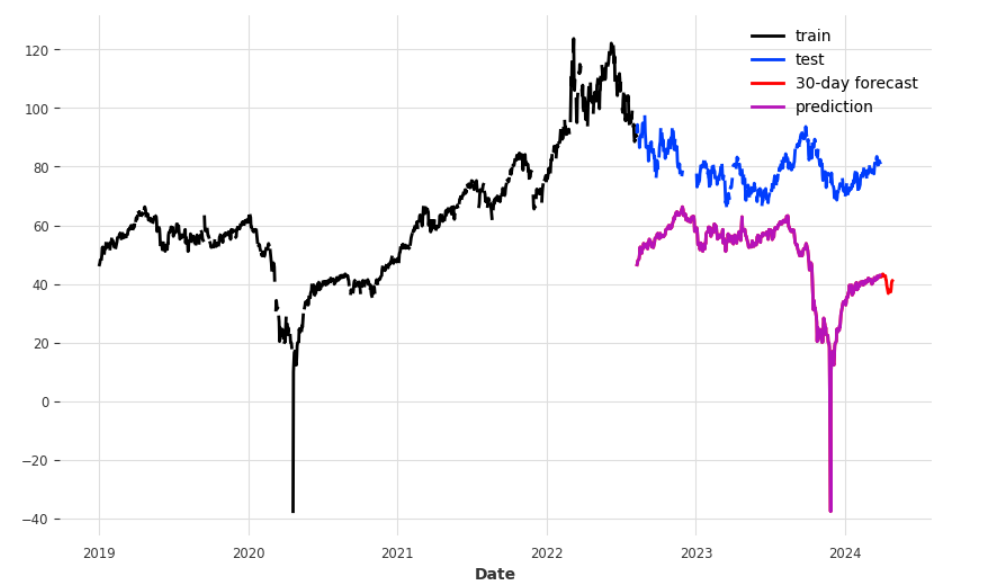
\includegraphics[width=0.8\textwidth]{Picture/FFT/crude.png} 
    \caption{Crude Oil WTI 7:3}
    \label{fig:1}
    \end{minipage}
    \hfill
    \\
    \begin{minipage}{0.3\textwidth} 
    \centering
    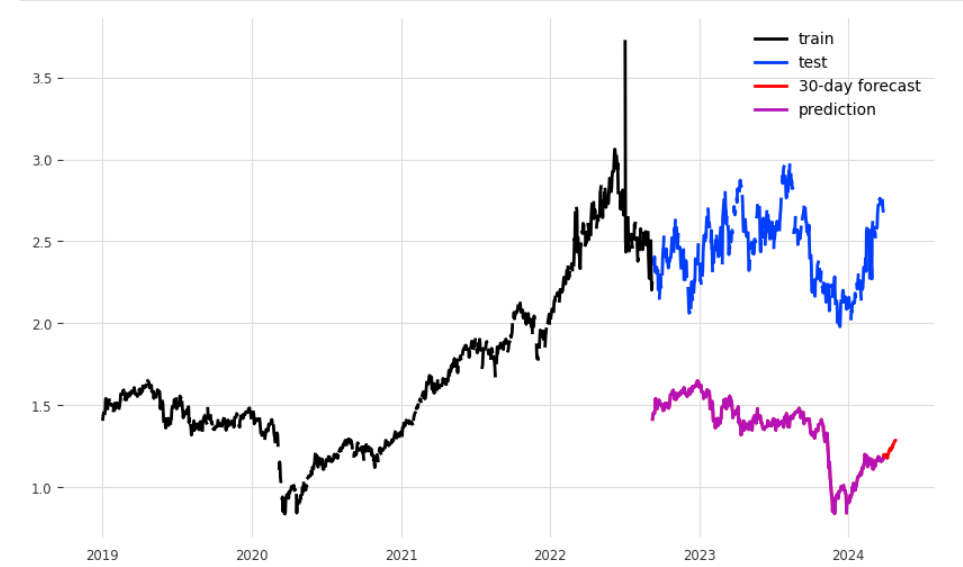
\includegraphics[width=0.8\textwidth]{Picture/FFT/gasoline.png}
    \caption{Gasoline RBOB 7:3}
    \label{fig:2}
    \end{minipage}
    \hfill
    \\
    \begin{minipage}{0.3\textwidth}
    \centering
    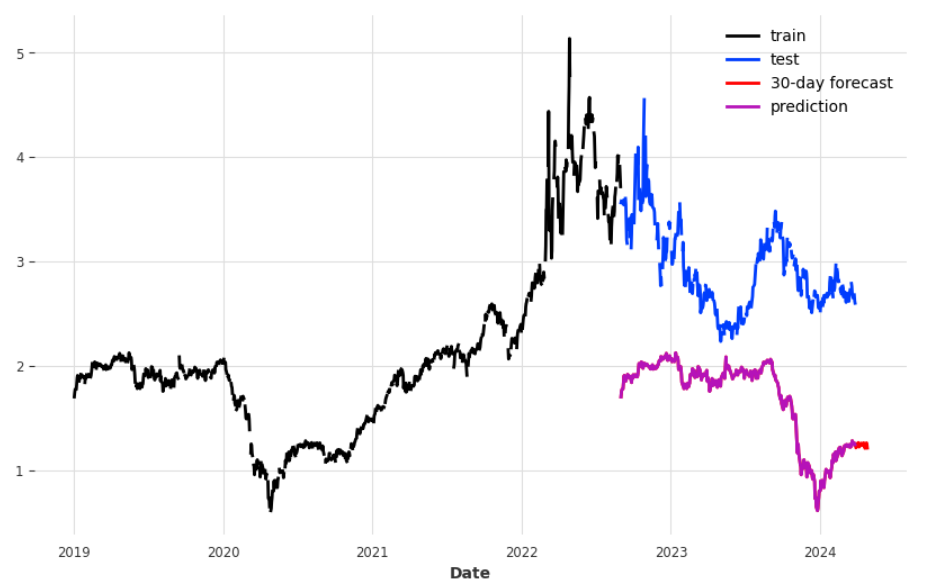
\includegraphics[width=0.8\textwidth]{Picture/FFT/Heating.png}
    \caption{Heating Oil 7:3}
    \label{fig:3}
    \end{minipage}
\end{figure}

\subsection{Random Forest (RF)}
Random Forest là một phương pháp học máy phổ biến được sử dụng vì tính linh hoạt, đơn giản và thường mang lại hiệu quả cao. Về bản chất thì Random Forest là tập hợp của nhiều cây quyết định, thay vì phụ thuộc vào một cây, nó lấy dự đoán từ mỗi cây và dựa trên đa số phiếu dự đoán, để đưa ra kết quả cuối cùng.

Dưới đây là sơ đồ minh họa cho Xây dựng Cây quyết định:

\begin{figure}[H]
    \centering
    \begin{minipage}{0.3\textwidth}
    \centering
    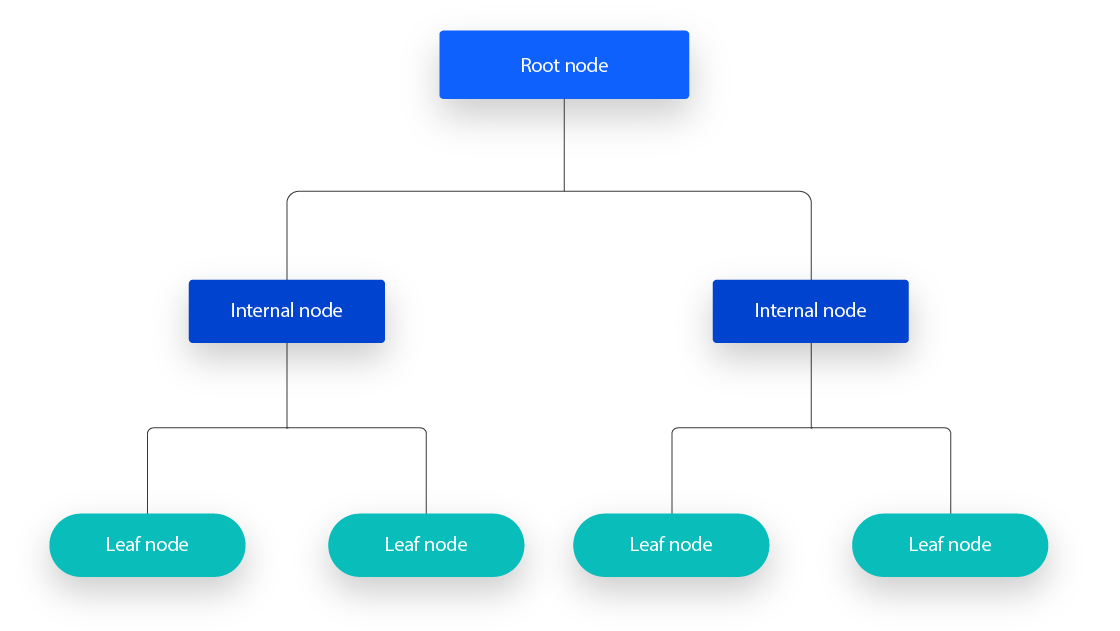
\includegraphics[width=0.8\textwidth]{Picture/RF/Decision-Tree.png} 
    \caption{Mô hình cây quyết định (Decision Tree)}
    \label{fig:1}
    \end{minipage}
    \hfill
    \\
  
\end{figure}

Một cây quyết định được tạo thành từ ba loại nút:

• Nút quyết định : Loại nút này có hai nhánh trở lên.

• Các nút lá : Các nút thấp nhất đại diện cho quyết định.

• Nút gốc : Đây cũng là nút quyết định nhưng ở cấp cao
nhất.


Random Forest là một thuật toán học có giám sát có thể giải
quyết cả các vấn đề phân loại và hồi quy. Nó hoạt động theo bốn bước:

1. Chọn mẫu ngẫu nhiên từ tập dữ liệu cho trước.

2. Thiết lập một cây quyết định cho mỗi mẫu và nhận kết
quả dự đoán từ mỗi cây quyết định.

3. Sau đó, bỏ phiếu cho mỗi kết quả dự đoán.

4. Chọn kết quả được dự đoán nhiều nhất là kết quả dự
đoán cuối cùng.

Dưới đây là mô hình của Random Forest:

\begin{figure}[H]
    \centering
    \begin{minipage}{0.3\textwidth}
    \centering
    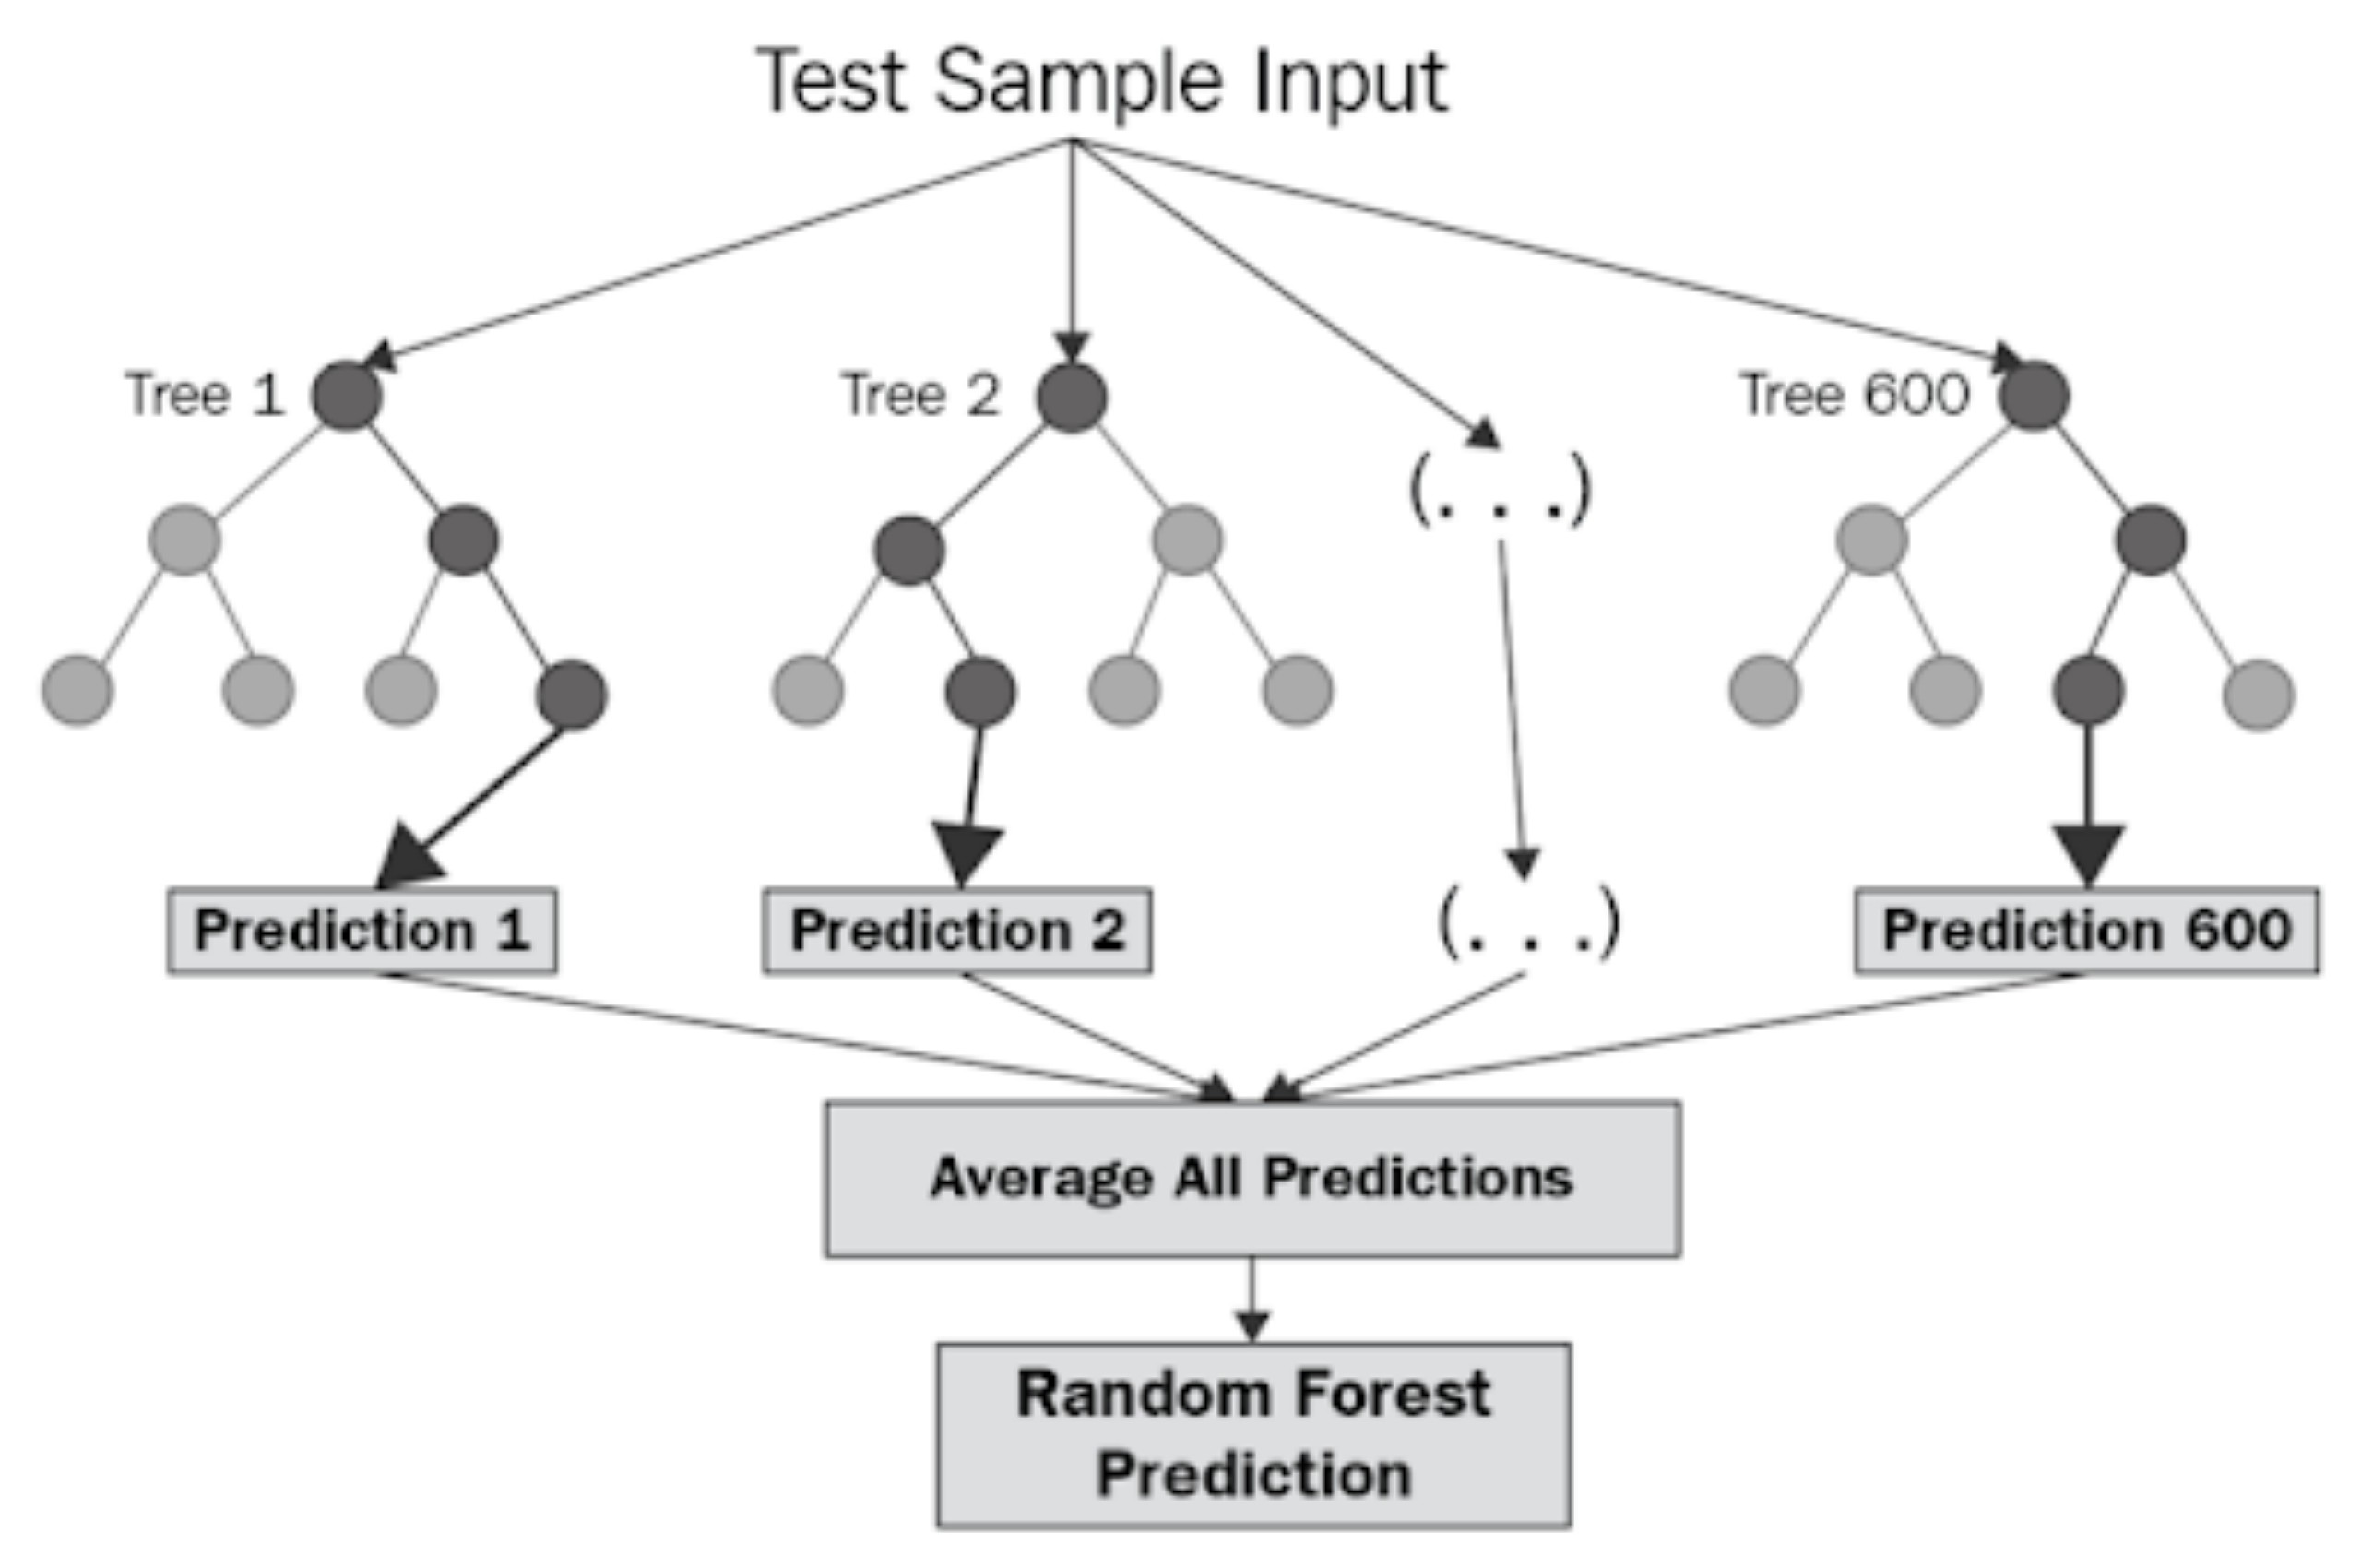
\includegraphics[width=0.8\textwidth]{Picture/RF/RF_Model.jpg} 
    \caption{Mô hình Random Forest}
    \label{fig:1}
    \end{minipage}
    \hfill
    \\
  
\end{figure}

\begin{figure}[H]
    \centering
    \begin{minipage}{0.3\textwidth}
    \centering
    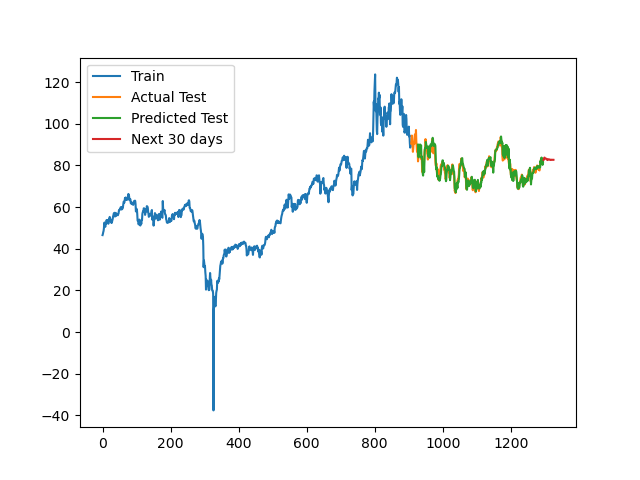
\includegraphics[width=0.8\textwidth]{Picture/RF/Cruide_Oil_73_Fix.png} 
    \caption{RF Crude Oil WTI 7:3}
    \label{fig:1}
    \end{minipage}
    \hfill
    \\
    \begin{minipage}{0.3\textwidth} 
    \centering
    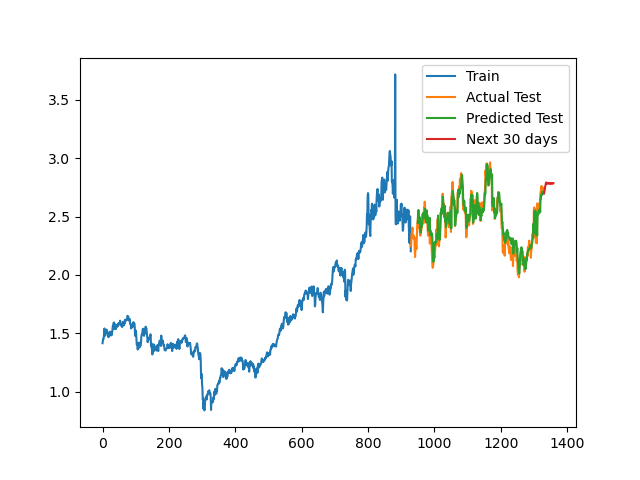
\includegraphics[width=0.8\textwidth]{Picture/RF/Gasoline_RBOB_73_Fix.png}
    \caption{RF Gasoline RBOB 7:3}
    \label{fig:2}
    \end{minipage}
    \hfill
    \\
    \begin{minipage}{0.3\textwidth}
    \centering
    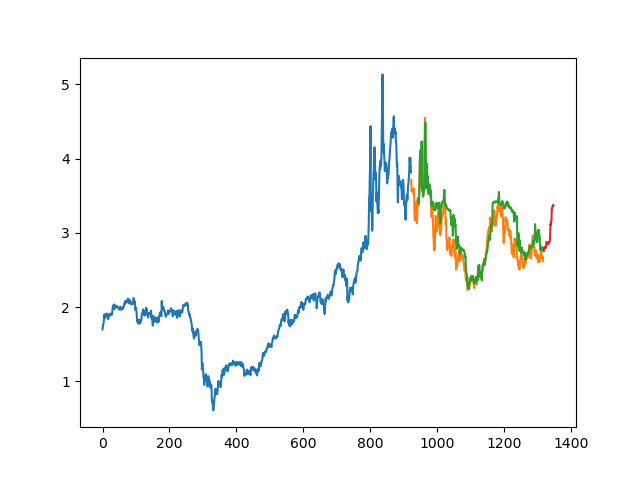
\includegraphics[width=0.8\textwidth]{Picture/RF/Heating_Oil_73_Fix.png}
    \caption{RF Heating Oil 7:3}
    \label{fig:3}
    \end{minipage}
\end{figure}

\subsection{Dynamic Linear Model (DLM)}
Mô hình tuyến tính động (Dynamic Linear Model - DLM) là một thuật toán thống kê được sử dụng để mô hình hóa và dự đoán các chuỗi dữ liệu thời gian. Nó là một phần của lĩnh vực học máy thống kê và thường được sử dụng trong việc phân tích dữ liệu thời gian, dự báo, và điều khiển.
Một DLM bao gồm hai thành phần chính:
\begin{itemize}
    \item State component: Đây là một mô hình tuyến tính động mà mô tả sự phát triển của hệ thống theo thời gian. Thông thường, mô hình trạng thái sử dụng một số biến trạng thái để mô hình hóa sự biến đổi và sự phụ thuộc của dữ liệu thời gian. Mô hình trạng thái thường được mô tả bằng một phương trình đệ quy.
    \item Observation component: Đây là mô hình mô tả cách các biến quan sát được tạo ra từ các biến trạng thái. Thông thường, mô hình quan sát sử dụng một mô hình tuyến tính để liên kết giữa các biến trạng thái và các biến quan sát.
\end{itemize}
Phương trình trạng thái (State equation):
\begin{equation}
\mathbf{x}_t = \mathbf{G}_t \mathbf{x}_{t-1} + \mathbf{w}_t
\end{equation}
Trong đó:
\begin{itemize}
    \item $\mathbf{x}_t$ là vector trạng thái tại thời điểm $t$.
    \item $\mathbf{G}_t$ là ma trận chuyển tiếp trạng thái tại thời điểm $t$.
    \item $\mathbf{w}_t$ là vecto nhiễu trạng thái tại thời điểm $t$.
\end{itemize}
Phương trình quan sát (Observation equation)::
\begin{equation}
\mathbf{y}_t = \mathbf{F}_t \mathbf{x}_t + \mathbf{v}_t
\end{equation}
Trong đó:
\begin{itemize}
    \item $\mathbf{y}_t$ là vector quan sát tại thời điểm $t$.
    \item $\mathbf{F}_t$ là ma trận quan sát tại thời điểm $t$.
    \item $\mathbf{v}_t$ là vecto nhiễu quan sát tại thời điểm $t$.
\end{itemize}
\begin{figure}[H]
    \centering
    \begin{minipage}{0.3\textwidth}
    \centering
    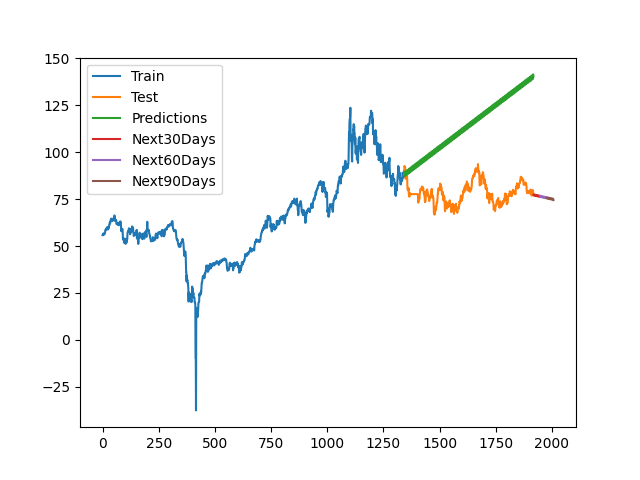
\includegraphics[width=0.8\textwidth]{Picture/DLM/crude.png} 
    \caption{Crude Oil WTI 7:3}
    \label{fig:1}
    \end{minipage}
    \hfill
    \\
    \begin{minipage}{0.3\textwidth} 
    \centering
    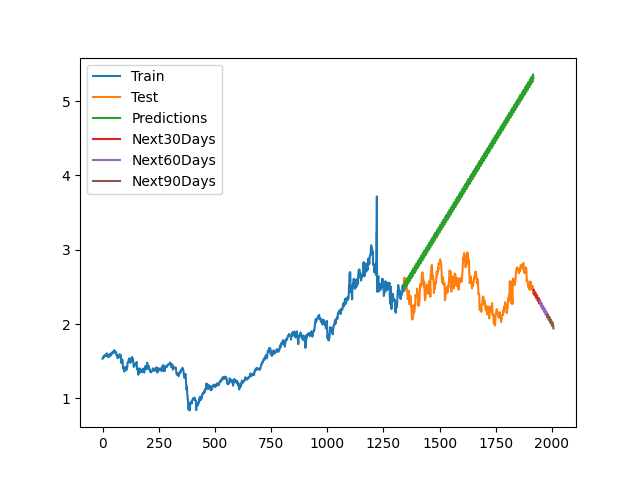
\includegraphics[width=0.8\textwidth]{Picture/DLM/gasoline.png}
    \caption{Gasoline RBOB 7:3}
    \label{fig:2}
    \end{minipage}
    \hfill
    \\
    \begin{minipage}{0.3\textwidth}
    \centering
    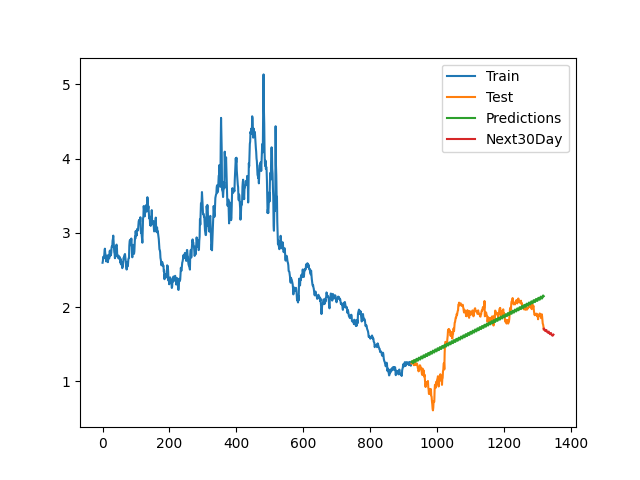
\includegraphics[width=0.8\textwidth]{Picture/DLM/heating.png}
    \caption{Heating Oil 7:3}
    \label{fig:3}
    \end{minipage}
\end{figure}
\subsection{Long short-term memory (LSTM)}
LSTM là một loại đặc biệt của RNN với các tính năng bổ sung để ghi nhớ chuỗi dữ liệu. Việc ghi nhớ xu hướng trước đó của dữ liệu là có thể thông qua một số cổng cùng với một dòng bộ nhớ được tích hợp trong một LSTM điển hình.  

Hình dưới đây biểu diễn khối bộ nhớ của LSTM:
\begin{figure}[H]
    \centering
    \begin{minipage}{0.3\textwidth}
    \centering
    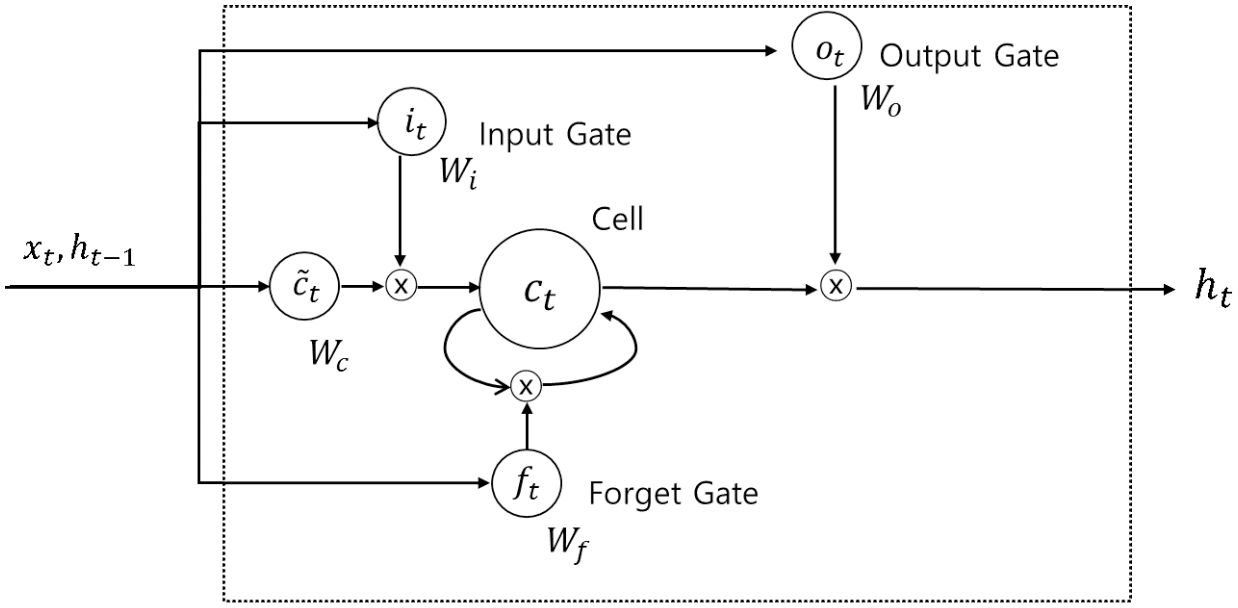
\includegraphics[width=0.8\textwidth]{Picture/LSTM/LSTM_pic.png} 
    \caption{Khối bộ nhớ của một LSTM}
    \label{fig:1}
    \end{minipage}
    \hfill
    \\
  
\end{figure}

Ba loại cổng được tham gia vào mỗi LSTM với mục tiêu kiểm soát trạng thái của từng ô:

\begin{itemize}
    \item Cổng Quên xuất ra một số giữa 0 và 1, trong đó 1 cho thấy "hoàn toàn giữ lại điều này"; trong khi 0 ngụ ý "hoàn toàn bỏ qua điều này".
    \item Cổng Bộ Nhớ chọn dữ liệu mới nào cần được lưu trữ trong ô. Đầu tiên, một lớp sigmoid, được gọi là "lớp cửa vào" chọn những giá trị nào sẽ được thay đổi. Tiếp theo, một lớp "tanh" tạo ra một vector các giá trị ứng viên mới có thể được thêm vào trạng thái.
    \item Cổng Đầu Ra quyết định những gì sẽ được xuất ra từ mỗi ô. Giá trị xuất ra sẽ dựa trên trạng thái ô cùng với dữ liệu được lọc và thêm mới. 
\end{itemize}

 Cụ thể, biểu thức toán học của LSTM được viết như sau:
 
1. Cổng Quên:
\begin{equation}
f_t = \sigma(W_{xf} x_t + W_{hf} h_{t-1} + b_f)
\end{equation}

2. Cổng Bộ Nhớ:
\begin{equation}
i_t = \sigma(W_{xi} x_t + W_{hi} h_{t-1} + b_i)
\end{equation}

3. Giá trị ứng viên mới:
\begin{equation}
\tilde{c}_t = \tanh(W_{xc} x_t + W_{hc} h_{t-1} + b_c)
\end{equation}

4. Trạng thái ô hiện tại:
\begin{equation}
c_t = f_t \ast c_{t-1} + i_t \ast \tilde{c}_t
\end{equation}

5. Cổng Đầu Ra:
\begin{equation}
o_t = \sigma(W_{xo} x_t + W_{ho} h_{t-1} + b_o)
\end{equation}

6. Đầu ra ô:
\begin{equation}
h_t = o_t \ast \tanh(c_t)
\end{equation}

Trong đó:
- \( \sigma \) là hàm sigmoid

- \( \tanh \) là hàm hyperbolic tangent

- \( W \) là các ma trận trọng số

- \( b \) là các hệ số bù

- \( x_t \) là đầu vào tại thời điểm \( t \)

- \( h_{t-1} \) là đầu ra của ô tại thời điểm \( t-1 \)

- \( c_t \) là trạng thái ô tại thời điểm \( t \)

- \( f_t \) là đầu ra của cổng quên

- \( i_t \) là đầu ra của cổng bộ nhớ

- \( o_t \) là đầu ra của cổng đầu ra

- \( \tilde{c}_t \) là giá trị ứng viên mới cho trạng thái ô

Trong các phương trình (1) đến (6), các biến đầu vào \( x_t \) và \( h_{t-1} \) đi vào bốn cổng được gán nhãn là \( f_t \), \( i_t \),\( c_t \), \( o_t \). Đối với các cổng đầu vào và đầu ra, các trọng số tương ứng với mỗi cổng được tính toán, và hàm sigmoid được sử dụng làm hàm kích hoạt. Hàm sigmoid lấy giá trị giữa 0 và 1. Nếu giá trị đầu ra là 1, giá trị tương ứng nên được giữ lại, nhưng nếu giá trị đầu ra là 0, giá trị tương ứng nên bị loại bỏ hoàn toàn. Đối với cổng còn lại, cổng điều chế đầu vào, hàm tanh được sử dụng để xác định lượng thông tin mới cần được phản ánh trong trạng thái ô. Cuối cùng, thông tin cần được phản ánh trong \( c_t \) được tính bằng cách cộng nhân điểm của các giá trị \( i_t \) đã tính toán trước đó và các giá trị được tính từ cổng quên, giá trị trạng thái ô trước đó, và nhân điểm của \( c_t \). Cuối cùng, để tính giá trị đầu ra \( h_t \), nhân điểm được thực hiện trên giá trị được tính từ cổng đầu ra và giá trị thu được bằng cách thêm hàm tanh vào giá trị trạng thái ô đã tính toán.



\section*{Acknowledgment}

The preferred spelling of the word ``acknowledgment'' in America is without 
an ``e'' after the ``g''. Avoid the stilted expression ``one of us (R. B. 
G.) thanks $\ldots$''. Instead, try ``R. B. G. thanks$\ldots$''. Put sponsor 
acknowledgments in the unnumbered footnote on the first page.

\section*{References}

Please number citations consecutively within brackets \cite{b1}. The 
sentence punctuation follows the bracket \cite{b2}. Refer simply to the reference 
number, as in \cite{b3}---do not use ``Ref. \cite{b3}'' or ``reference \cite{b3}'' except at 
the beginning of a sentence: ``Reference \cite{b3} was the first $\ldots$''

Number footnotes separately in superscripts. Place the actual footnote at 
the bottom of the column in which it was cited. Do not put footnotes in the 
abstract or reference list. Use letters for table footnotes.

Unless there are six authors or more give all authors' names; do not use 
``et al.''. Papers that have not been published, even if they have been 
submitted for publication, should be cited as ``unpublished'' \cite{b4}. Papers 
that have been accepted for publication should be cited as ``in press'' \cite{b5}. 
Capitalize only the first word in a paper title, except for proper nouns and 
element symbols.

For papers published in translation journals, please give the English 
citation first, followed by the original foreign-language citation \cite{b6}.


\begin{thebibliography}{00}
\bibitem{b1} T. Gopalakrishnan, R. Choudhary, and S. Prasad, "Prediction of Sales Value in Online shopping using Linear Regression," in 2018 4th International Conference on Computing Communication and Automation (ICCCA), 2018, pp. 1-6.
\bibitem{b2} Benvenuto, D., Giovanetti, M., Vassallo, L., Angeletti, S., & Ciccozzi, M. (2020). Application of the ARIMA model on the COVID-2019 epidemic dataset. Data in brief, 29, 105340.
\bibitem{b3} Belavadi, S. V., Rajagopal, S., Ranjani, R., & Mohan, R. (2020). Air quality forecasting using LSTM RNN and wireless sensor networks. Procedia Computer Science, 170, 241-248.
\bibitem{b4} Kisvari, A., Lin, Z., & Liu, X. (2021). Wind power forecasting–A data-driven method along with gated recurrent neural network. Renewable Energy, 163, 1895-1909.
\bibitem{b5} P Sun, N AlJeri, A Boukerche - 2018. A fast vehicular traffic flow prediction scheme based on fourier and wavelet analysis.
\bibitem{b6} K. V. Narasimha Murthy, G. Kishore Kumar & P. N (2024). Sen Dynamic Linear Modeling for Characterizing and Predicting the Patterns of Summer Monsoon Rainfall in Northwest India.
\bibitem{b7} C. Hecht; R. Aghsaee; F. Schwinger; J. Figgener; M. Jarke; D. U. Sauer (2022). Short-term prediction of electric vehicle charging station availability using cascaded machine learning models.
.
\bibitem{b8}  Neelamadhab Padhy, Srinivasarao Dharmireddi, Dushmanta Kumar Padhy, R. Saikrishna & K. Srujan Raju (2023).Stock Market Prediction Performance Analysis by Using Machine Learning Regressor Techniques.

\end{thebibliography}
\vspace{12pt}


\end{document}
